\documentclass[10pt, twoside]{book}
    %\usepackage[chinese]{babel}
    \usepackage[utf8]{inputenc}
    \usepackage[T1]{fontenc}
%%%%% Pacchetti
\usepackage{FileAusiliari/Layout}			% Contiene i pacchetti e le impostazioni per il layout
\usepackage{FileAusiliari/Pacchetti}		% Pacchetti aggiuntivi di vario tipo (senza tikz)
\usepackage{FileAusiliari/TikZ}				% Ambiente tikzpicture
\usepackage{FileAusiliari/Definizioni}		% Definizioni di colori, variabili globali ecc.
\usepackage{FileAusiliari/Environments}		% Impostazioni TOC, bibliografia e indice analitico + environments vari per il contenuto del documento
\usepackage{FileAusiliari/Custom}			% Tutto ciò che è personalizzabile normalmente dall'utente (tranne i colori per collegamenti ipertestuali, citazioni, link, che sono da modificare in Referencing)
%%%%%%%%%% Impostazioni indice analitico
%%%%%%%%%%%%%%%%%%%%%%%%%%%%%%%%%%%%
\usepackage{imakeidx}
\indexsetup{othercode=\small}
\makeindex[columns=2, intoc=false, columnseprule, title={}, 
           options= -s FileAusiliari/Stile.ist]
%%%%%%%%%%									Collegamenti ipertestuali
%%%%%%%%%%
\RequirePackage[breaklinks, colorlinks=true, hypertexnames=true, linktoc=all]{hyperref}

	%%%%%%%%%% Colori dei link ipertestuali
	\hypersetup{colorlinks, %I colori sono per il pdf, per la stampa impostare 'black' per tutti i colori
			urlcolor={Url},  % default='Url'
			citecolor={Cite}, % default='Cite'
			linkcolor={Link}} % default='Link'

%%% Miglior referencing
\pagenumbering{none}		% Collegamenti ipertestuali e indice analitico
\usepackage{FileAusiliari/Comandi}			% Comandi vari
\usepackage{fancyhdr}
\usepackage{titlesec}
\usepackage{listings}
\usepackage{graphicx}
\usepackage{caption}
\usepackage{hyperref}
\usepackage{makeidx}
\usepackage{xcolor}
\usepackage{multirow}

\usepackage{fontspec} % 字體
\usepackage{xeCJK}    % 中文支持
\setmainfont{Times New Roman} % 主字體
\setCJKmainfont{Noto Sans CJK TC} % 中文黑體 思源黑體
\linespread{1.5}

\newcommand{\CJKsection}[1]{{\CJKfamily{titlefont}#1}} % 中文支持 Section Title

\titleformat{\section}{\Large\bfseries\CJKsection}{\thesection}{1em}{}
\titleformat{\subsection}{\large\bfseries\CJKsection}{\thesubsection}{1.5em}{}
\titleformat{\subsubsection}{\normalsize\bfseries\CJKsection}{\thesubsubsection}{2em}{}



% 自定義命令
\newcommand{\code}[1]{\texttt{#1}}
\newcommand{\term}[1]{\textit{#1}}
\renewcommand{\bold}[1]{\textbf{#1}}
\newcommand{\figref}[1]{\textbf{Figure~\ref{#1}}}
\newcommand{\tabref}[1]{\textbf{Table~\ref{#1}}}
\newcommand{\lstref}[1]{\textbf{Listing~\ref{#1}}}
\newcommand{\chapref}[1]{\textbf{Chapter~\ref{#1}}}
\newcommand{\secref}[1]{\textbf{Section~\ref{#1}}}


\definecolor{codegreen}{rgb}{0,0.6,0}
\definecolor{codegray}{rgb}{0.5,0.5,0.5}
\definecolor{codepurple}{rgb}{0.58,0,0.82}
\definecolor{backcolour}{rgb}{0.95,0.95,0.92}
\lstdefinestyle{mystyle}{
  backgroundcolor=\color{backcolour}, commentstyle=\color{codegreen},
  keywordstyle=\color{magenta},
  numberstyle=\tiny\color{codegray},
  stringstyle=\color{codepurple},
  basicstyle=\ttfamily\footnotesize,
  breakatwhitespace=false,         
  breaklines=true,                 
  captionpos=t,                    
  keepspaces=true,                 
  numbers=left,                    
  numbersep=5pt,                  
  showspaces=false,                
  showstringspaces=false,
  showtabs=false,                  
  tabsize=2
}
\lstset{style=mystyle}


%%%%%%%%%%%%%%%%%%%%%%%%%%%%
%%%%%%%%%%%%%%%%%%%%%%%%%%%%
\begin{document}
%%%%%%%%%%%%%%%%%%%%%%%%%%%%									 TITOLO
%%%%%%%%%%%%%%%%%%%%%%%%%%%%
% \begin{titlepage}
    \raggedleft	
    \rule{1pt}{.125\textheight}
	\hspace{0.025\textwidth}
	\parbox[b]{.85\textwidth}{
		{\HUGE\bfseries Titolo (versione 1)
        }\\[2\baselineskip]
		{\Large\textit{Sottotitolo}}\\[45.5\baselineskip]
        {\Large\textsc{Mattia Puddu}\\[.35\baselineskip] mattiapuddu@icloud.com} \\\\\\\\
        %{\Large\textit{Mattia Puddu (seconda versione)}}\\
        {\Large\today}

 }
\end{titlepage}
\begin{titlepage}

% % LOGO
% \begin{figure}[ht]\centering
%     
\includegraphics[scale=.6]{FileAusiliari/Logo/MarchioBlack.pdf}
% \end{figure}

% TITLE AND SUBTITLE
\vspace{2.5cm}
\parbox[l]{.9\textwidth}{\centering
    {\HUGE \bfseries 使用 HIP 的加速運算}\\[2\baselineskip]
    {\Large \textit{加速運算技術與應用研究}}\\[.5\baselineskip]}

\vspace*{\fill}

% AUTHOR
\parbox[b]{.5\textwidth}{
    \rule{1pt}{.125\textheight}
    \hspace{0.025\textwidth}
    \parbox[b]{.8\textwidth}{
        {\Large \bfseries 作者}\\[1\baselineskip]
        {\Large \textsc{Yifan Sun, Sabila Al Jannat, \\ Trinayan Baruah, and David Kaeli}}\\[2\baselineskip]
        {\Large 2024 年 10 月}
    }
}
\parbox[b]{.5\textwidth}{
    \rule{1pt}{.125\textheight}
    \hspace{0.025\textwidth}
    \parbox[b]{.8\textwidth}{
        {\Large \bfseries 翻譯}\\[1\baselineskip]
        {\Large \textsc{牟展佑、程詩柔、謝之豫、牟懋軒\\林展毅、黃煒智、魏士勛、白宸安\\郭品毅、周志遠}}\\[1\baselineskip]
        {\Large 2025 年 7 月}
    }
}
\end{titlepage}

%%%%%%%%%%%%%%%%%%%%%%%%%%%%									FRONTMATTER
%%%%%%%%%%%%%%%%%%%%%%%%%%%%
\frontmatter
\pagestyle{fancyfront}
%%%%%								 INDICE
\begingroup
{
	\let\cleardoublepage\relax
	%%%%%		Nome Indice (NASCOSTO E CREATO A PARTE)
	\renewcommand\contentsname{}
	\begin{tikzpicture}[remember picture, overlay]
		\clip (-80,-95) rectangle (40,10);
		\pgftext[x=.8\textwidth, y=0.2cm]{\HUGE\bfseries 
		目錄}						% Titolo indice
		\end{tikzpicture}
	\vspace{-1cm}
	
	\tableofcontents
	\vspace{.25cm}
}
%%%%%								INTRODUZIONE
		\titleformat{\chapter}
		[hang]
		{\Huge}
		{}
		{0em}
		{}
		[\Large {\begin{tikzpicture} [remember picture, overlay]
		\pgftext[right,x=14.75cm,y=0.2cm]{\HUGE\bfseries 
			前言}
		\end{tikzpicture}}]
%%%%%%%%%%%%%%%%%%%%%%%%%%%%%%%%%%%%%%%%%%%%%%%%%%%%%%%%%%%%%%%%%%%%%%%%%%%%%%%%%
\chapter*{}\normalfont\addcontentsline{toc}{part}{前言}

高效能運算(High-Performance Computing, HPC)的世界最近見證了一個重要里程碑,即在美國橡樹嶺國家實驗室(Oak Ridge National Laboratory)部署的 \textbf{Frontier 超級電腦}首次達成 \textbf{Exascale} 性能。隨著計算性能的此項突破,一類全新的應用場景得以實現,包括:
\begin{itemize}
    \item 天氣與氣候預測,
    \item 生物醫學研究,
    \item 高端設備開發,
    \item 新能源研究與探索,
    \item 動畫設計,
    \item 新材料研究,
    \item 工程設計、模擬與分析,
    \item 遙測數據處理,以及
    \item 金融風險分析。
\end{itemize}

\textbf{AMD} 透過提供一系列高效能的 \textbf{CPU} 和 \textbf{GPU},以及支持 \textbf{HIP} 和 \textbf{ROCm} 執行的開源軟體堆棧,推動了這些進展的實現。這個新興的程式設計生態系統提供了許多創新的功能,包括硬體加速器(如 \textbf{AMD} 和 \textbf{NVIDIA GPU})的互操作性,以及對關鍵高效能編譯器(如 \textbf{LLVM})、叢集部署及核心應用框架(如 \textbf{Raja}、\textbf{Kokkos}、\textbf{TensorFlow} 和 \textbf{PyTorch})的支持,還包含多項高效能函式庫(如 \textbf{rocBLAS}、\textbf{rocSparse}、\textbf{MIOpen}、\textbf{RCCL} 和 \textbf{rocFFT})。

為配合這些進步,高效能運算社群也對此里程碑作出了貢獻,提供了最先進的第三方工具,用於性能監控、除錯器,以及視覺化工具。

由 \textbf{Yifan Sun}、\textbf{Sabila Al Jannat}、\textbf{Trinayan Baruah} 和 \textbf{David Kaeli} 共同撰寫的《\textit{Accelerated Computing with HIP}》第二版,為高效能運算社群提供了一份具參考價值的指南,幫助程式開發人員充分利用 \textbf{Exascale} 計算的優勢。該書內容涵蓋以下主題:


		\titleformat{\chapter}
		[hang]
		{\Huge}
		{}
		{0em}
		{}
		[\Large {\begin{tikzpicture} [remember picture, overlay]
		\pgftext[right,x=14.75cm,y=0.2cm]{\HUGE\bfseries 
			書寫規範}
		\end{tikzpicture}}]

\titlespacing*{\chapter}{0pt}{-30pt}{20pt}

%%%%%%%%%%%%%%%%%%%%%%%%%%%%%%%%%%%%%%%%%%%%%%%%%%%%%%%%%%%%%%%%%%%%%%%%%%%%%%%%%
\chapter*{}\normalfont\addcontentsline{toc}{part}{書寫規範}

% ======================
% 技術書寫規範
% ======================


\section*{文件結構}
\begin{itemize}
    \item 每章使用獨立的 \code{.tex} 文件,主文件透過 \code{\textbackslash input} 引入。
    \item 主文件負責樣式與章節組織,章節文件只包含內容。
\end{itemize}


\section*{字體命令}
\begin{itemize}
    \item \code{\textbackslash code\{example\}}:程式碼 ex: \code{printf}
    \item \code{\textbackslash term\{斜體術語\}}:斜體術語 ex: \term{example}。
    \item \code{\textbackslash bold\{粗體術語\}}:粗體術語 ex: \bold{example}。
\end{itemize}


\section*{引用命令}
\begin{itemize}
    \item \code{\textbackslash figref\{fig:example\}}:引用圖片。
    \item \code{\textbackslash tabref\{tab:example\}}:引用表格。
    \item \code{\textbackslash lstref\{lst:example\}}:引用程式碼塊。
    \item \code{\textbackslash chapref\{chapter\}}:引用 Chapter。
    \item \code{\textbackslash secref\{section\}}:引用 Section。
    
\end{itemize}

\section*{程式碼模板(看左邊 code)}
\begin{lstlisting}[language=Python, caption={範例程式碼:Python 計算平方值}, label={lst:example}]
def square(x):
    return x * x
\end{lstlisting}

\section*{補充}
\begin{itemize}
    \item 專有名詞大寫,注意英文複數。
    \item 等寬字體中英文間要空格。
    \item 中文為主的語句使用中文標點符號,如輝達(NVIDIA)。英文為主使用英文標點。
    \item 術語在第一次用到時需要用(English)來表明原文。
    \item 專有名詞翻譯依照 https://terms.naer.edu.tw/ 及 https://hackmd.io/@l10n-tw/glossaries 為準
\end{itemize}

\endgroup

%%%%%								ERRATA 
\iffalse
		\titleformat{\chapter}
		[hang]
		{\huge}
		{}
		{0em}
		{}
		[\large {\begin{tikzpicture} [remember picture, overlay]
		\pgftext[right,x=14.75cm,y=0.2cm]{\color{black}\Huge\bfseries 
			Errata corrige \& Aggiunte};
		\end{tikzpicture}}]
\chapter*{}\normalfont		\addcontentsline{toc}{part}{Errata corrige \& Aggiunte}
\begin{longtable}{p{2.55cm}p{1.45cm}p{9cm}}
	Data di \newline correzione & Pagina&\\\hline
	24/10/2023	& ?	& ?
\end{longtable}
\fi

%%%%%%%%%%%%%%%%%%%%%%%%%%%%									MAINMATTER
%%%%%%%%%%%%%%%%%%%%%%%%%%%%
\mainmatter

\pagestyle{fancymain}
\titleformat{\chapter}[display]{\bfseries\Large}	{\filleft\MakeUppercase{\chaptertitlename} \HUGE\thechapter}{.5ex}{\titlerule\vspace{1ex}\filleft}[\vspace{3.5ex}]
\titlespacing*{\chapter}{0pt}{0.1\baselineskip}{0.5\baselineskip}

\fancyheadoffset[L]{\dimexpr\oddsidemargin-0in\relax}
\fancyheadoffset[R]{\dimexpr\oddsidemargin-0in\relax}

\normalfont
\normalsize


% \newgeometry{top=35mm, bottom=35mm, left=15mm, right=15mm, headheight=0pt, headsep=0pt, marginparsep=0pt, marginparwidth=0pt, footskip=0pt, footnotesep=0pt}
% % \part*{\HUGE Parte 1}\label{Parte1}
% \restoregeometry

%%%%%								CAPITOLI
\input{Chapters/Chap1}
\input{Chapters/Chap2}
\input{Chapters/Chap3}
\input{Chapters/Chap4}
\input{Chapters/Chap5}
\input{Chapters/Chap6}
\input{Chapters/Chap7}
\input{Chapters/Chap8}
\input{Chapters/Chap9}
\input{Chapters/Chap10}
\input{Chapters/Chap11}
\input{Chapters/Chap12}
\input{Chapters/Chap13}



%%%%%								APPENDICI
\newgeometry{top=35mm, bottom=35mm, left=15mm, right=15mm, headheight=0pt, headsep=0pt, marginparsep=0pt, marginparwidth=0pt, footskip=0pt, footnotesep=0pt}
\part*{\HUGE Appendici}
\titleformat{\chapter}[display]    	{\bfseries\large\raggedright}    	{\vspace{-2.35cm} \MakeUppercase{\chaptertitlename}\ \Huge \thechapter}    	{.125ex}    	{\raggedleft\vspace{-1cm}\Huge\makebox[.5\textwidth]{}}
\titlespacing*{\chapter}{0pt}{6\baselineskip}{2.5\baselineskip}
\restoregeometry

	% Capitoli
\titlecontents{chapter}[2.5pc]
{\addvspace{15pt}}
{
\begin{tikzpicture}
		\pgftext{\LArge\bfseries\bfseries\color{black}\hspace{-1cm} Appendix \ \thecontentslabel{\color{white}.}\hspace{.5cm} }
	\end{tikzpicture}\Large }
{}
{\color{black}\titlerule\; \;\Large\bfseries Pagina \thecontentspage}

\pagestyle{fancyapp}

\begin{appendices}
	\chapter{ROCm 安裝指南}\label{AppendiceA}

在這個章節中,我們將介紹 ROCm 的安裝過程。安裝 ROCm 通常是使用 AMD GPU 的第一個步驟。因此,在開始開發或執行 GPU 程式之前,熟悉 ROCm 環境的安裝過程會有所幫助。

本章將介紹在 Ubuntu 20.04 LTS 作業系統上安裝 ROCm v5.4 的步驟。由於 ROCm 仍在積極開發,我們只會介紹所需的基本操作指令,並說明執行這些指令後的結果。隨著新版本的 ROCm 持續發布,本章部分內容可能會過時。因此,建議讀者在開始安裝之前,參考最新的安裝文件。ROCm 的安裝文件可在 \url{https://docs.amd.com} 取得。

\section{先備條件}

我們將示範如何在 Ubuntu 20.04 LTS 作業系統上安裝 ROCm。ROCm 可以支援多種不同的 Linux 作業系統發行版。目前 ROCm 並不支援 Microsoft Windows 作業系統,但 Windows 的支援可能會在近期推出。

ROCm 支援的作業系統如表格 \ref{table:rocm_supported_distros_and_kernel_versions} 所示。整體而言,ROCm 支援 Red Hat Enterprise Linux (RHEL)、SUSE Linux Enterprise Server (SLES) 和 Ubuntu 發行版。對於每個發行版,都有要求一個最低的核心版本(如 5.14, 4.18)。此外,系統上需要安裝一些額外的軟體套件,例如 \lstinline|wget|、\lstinline|gnupg2|、\lstinline|gawk| 和 \lstinline|curl|,因為這些是 ROCm 安裝腳本所需的必要工具。


\begin{table}[h!]
\centering
\caption{目前支援的 Linux 發行版與核心版本}
\label{table:rocm_supported_distros_and_kernel_versions}
\begin{tabular}{ll}
\hline
\textbf{作業系統} & \textbf{核心版本} \\ \hline  
RHEL 9.1 & 5.14 \\ 
RHEL 8.7 & 4.18 \\ 
RHEL 8.6 & 4.18 \\ 
SLES15 SP4 & 5.14.21 \\ 
Ubuntu 20.04.5 LTS & 5.15 \\ 
Ubuntu 22.04.1 LTS & 5.15, OEM 5.17 \\ \hline 
\end{tabular}
\end{table}


需要執行 GPU 程式的系統使用者必須加入適當的使用者群組。可以使用 groups 指令來檢查目前使用者所屬的群組。若要使用 GPU,使用者需加入 \lstinline|render| 或 \lstinline|video|(推薦)群組之一。可以使用指令 \lstinline|sudo usermod -a -G [群組名稱] [使用者名稱]| 來將使用者加入特定的群組。

在購買 GPU 硬體之前,應確認預計要購買的 GPU 是否被 ROCm 平台所之援(請參閱表格 \ref{table:rocm_supported_gpus})。

\begin{table}[h!]
\centering
\caption{ROCm 支援的 GPU 型號}
\label{table:rocm_supported_gpus}
\begin{tabular}{lll}
\hline
\textbf{GPU 系列} & \textbf{GPU} & \textbf{GFX ID} \\ \hline
\multirow{4}{*}{GCN} & AMD Radeon Instinct\texttrademark\ MI50 & \multirow{4}{*}{GFX906} \\ 
 & AMD Radeon Instinct\texttrademark\ MI60 & \\ 
 & AMD Radeon\texttrademark\ VII &  \\ 
 & AMD Radeon\texttrademark\ Pro VII &  \\ 
\multirow{2}{*}{RDNA} & AMD Radeon\texttrademark\ Pro W6800 & \multirow{2}{*}{GFX1030} \\ 
 & AMD Radeon\texttrademark\ Pro V620 &  \\ 
\multirow{2}{*}{CDNA} & AMD Instinct\texttrademark\ MI100 & GFX908 \\ 
 & AMD Instinct\texttrademark\ MI200 & GFX90a \\ \hline
\end{tabular}
\end{table}

\section{理解 ROCm 套件}

ROCm 是一個包含許多軟體套件的複雜生態系統。完整的套件列表可以參見圖 \ref{fig:rocm_packages}。這些套件可能有複雜的依賴性關係。為了避免使用者需要逐一安裝套件,ROCm 將這些套件分組為元套件 (meta-package)(完整列表請參見表格 \ref{table:rocm_meta_packages})。使用者通常會選擇安裝元套件,而非獨立安裝各個套件。

\begin{figure}
    \centering
    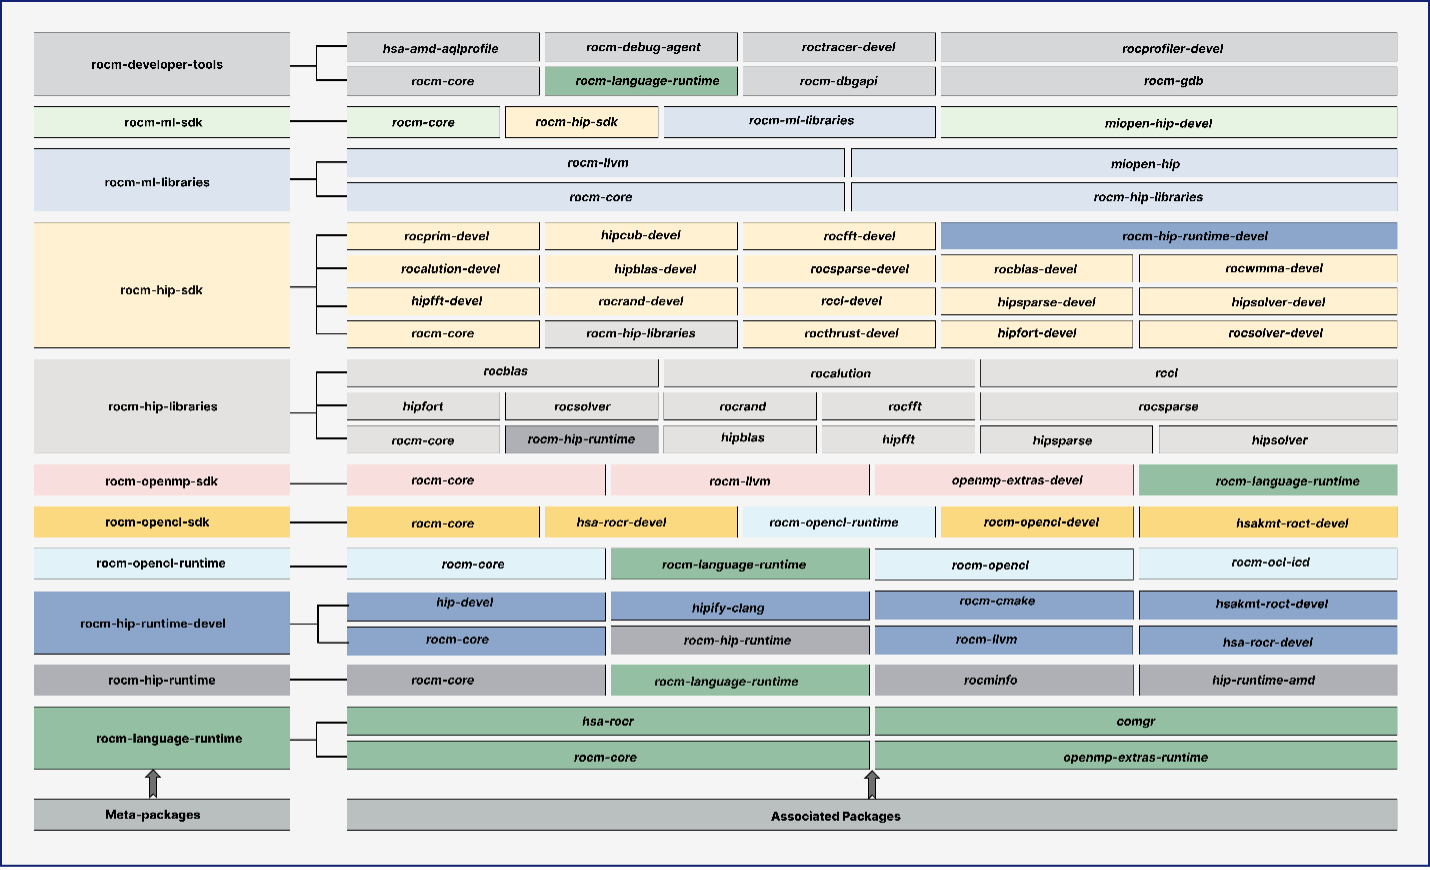
\includegraphics[width=1\linewidth]{Appendici/MetaPackages.png}
    \caption{ROCm 元套件的列表以及包含在元套件中的各個獨立套件}
    \label{fig:rocm_packages}
\end{figure}


\section{安裝}

在此概論中,我們介紹兩種安裝 ROCm 的方法,包含安裝程式腳本的方法與套件管理器的方法。

\subsection{安裝程式腳本方法}
\label{sec:rocm_installer_method}
安裝程式腳本方法自動化了 AMDGPU 和 ROCm 的安裝過程。安裝程式腳本會處理 ROCm 的完整安裝過程,包括設定儲存庫、清理檔案系統、更新和安裝所需的驅動程式與元套件。使用此方法,系統對 ROCm 安裝過程有更多控制權。因此,那些對標準 Linux 指令不太熟悉的使用者可以選擇此方法來安裝 ROCm。可以使用以下指令下載並安裝安裝程式:

\begin{lstlisting}[caption={使用安裝程式腳本安裝 ROCm 所需指令}, label={lst:a1}]
sudo apt-get update
wget https://repo.radeon.com/amdgpu-install/5.4.3/ubuntu/focal/amdgpu-install_5.4.50403-1_all.deb
sudo apt-get install ./amdgpu-install_5.4.50403-1_all.deb
\end{lstlisting}

上述指令應該會安裝一個可以幫助管理 ROCm 套件的 \lstinline|amdgpu-install| 程式。如要安裝 ROCm,我們可以使用 \lstinline|sudo ./amdgpu-install| 指令執行安裝。此外,使用者也可以透過像是 \lstinline|sudo amdgpu-install --usecase=rocm| 的指令來安裝特定的使用案例。如果使用者希望一次安裝多個使用案例,可以在 \lstinline|usecase| 參數中指定多個值,並以逗號分隔。例如,指令 \lstinline|sudo amdgpu-install --usecase=rocm,hiplibsdk| 會同時安裝 ROCm 和 \lstinline|hiplibsdk| 兩個使用案例。使用 \lstinline|sudo amdgpu-install --list-usecase| 可以顯示所有可用的使用案例的列表。


\subsection{套件管理器方法}

套件管理器方法提供使用者更多安裝選項的靈活性,但在安裝過程中需要更多的使用者操作。建議此方法僅供進階使用者使用。總體來說,使用套件管理器安裝 ROCm 包括以下六個步驟:

\paragraph{步驟 1:安裝 Linux 核心標頭與開發套件}
使用套件管理器方法的前置步驟之一是安裝正確的 Linux 核心標頭與開發套件。

可以使用指令 \lstinline!sudo dpkg -l | grep linux-headers! 來檢查已安裝的核心標頭版本。例如,輸出的結果可能是 \lstinline|ii linux-headers-5.15.0-41-generic 5.15.0-41.44 20.04.1 amd64 Linux kernel headers for version 5.15.0 on 64 bit x86 SMP|。
類似地,可以使用指令 \lstinline!sudo dpkg -l | grep linux-modules-extra! 來列出開發套件,在作者的系統中輸出的結果為
\lstinline|ii linux-modules-extra-5.15.0-41-generic 5.15.0-41.44 20.04.1 amd64 Linux kernel extra modules for version 5.15.0 on 64 bit x86 SMP|。
如果當前版本的 Linux 標頭不符合表 \ref{table:rocm_supported_distros_and_kernel_versions} 中列出的要求,使用者需要使用指令 \lstinline|sudo apt install linux-headers-$(uname -r) linux-modules-extra-$(uname -r)| 來安裝所需的 Linux 標頭。


\paragraph{步驟 2:安裝 AMD GPU 驅動程式}
接下來,我們會使用套件管理器安裝 AMD GPU 驅動程式。套件管理器要求套件必須加密,因此需要安裝一組 GNU Privacy Guard(GPG)金鑰。安裝 GPG 金鑰的指令為:

\lstinline!curl -fsSL https://repo.radeon.com/rocm/rocm.gpg.key | sudo gpg --dearmor -o /etc/apt/trusted.gpg.d/rocm-keyring.gpg!。

接下來,使用以下指令將 AMD GPU 儲存庫新增到 Ubuntu 的套件管理器中:

\lstinline!echo 'deb [arch=amd64 signed-by=/etc/apt/trusted.gpg.d/rocm-keyring.gpg] https://repo.radeon.com/amdgpu/5.4.3/ubuntu focal main' | sudo tee /etc/apt/sources.list.d/amdgpu.list!。
新增儲存庫後,別忘了執行 \lstinline|sudo apt-get update|,讓套件管理器能夠取得套件資訊。
最後,使用 \lstinline|sudo apt install amdgpu-dkms| 來安裝 AMD GPU 驅動程式。安裝完成後,需要重新啟動系統。

\paragraph{步驟 3:安裝 ROCm 環境}
為了安裝 ROCm 環境,我們需要使用以下指令將外部資源加入到 Ubuntu 的套件管理器中:

\lstinline!echo 'deb [arch=amd64 signed-by=/etc/apt/trusted.gpg.d/rocm-keyring.gpg] https://repo.radeon.com/rocm/apt/5.4.3 focal main' | sudo tee /etc/apt/sources.list.d/rocm.list!

此指令會建立 \lstinline|rocm.list|,其中包含提供套件的 URL。

接下來,我們需要透過以下指令修改優先權:

\lstinline!echo -e 'Package: *\nPin: release o=repo.radeon.com\nPin-Priority: 600' | sudo tee /etc/apt/preferences.d/rocm-pin-600! 

透過為 ROCm 套件設定較高的優先權,我們可以在更新套件時保持穩定版本的 Ubuntu。在新增套件來源並修改優先設定後,我們仍然需要執行 \lstinline|sudo apt-get update|。


\subsection{驗證安裝}
無論使用哪種安裝方法,我們都需要驗證安裝是否成功。如果執行過程中出現錯誤,使用者應該首先檢查 ROCm 安裝是否已損壞。

首先,我們可以檢查 \lstinline|/opt/rocm|目錄是否包含預期的執行檔,例如 \lstinline|rocm-smi|,以及 ROCm 函式庫,例如 \lstinline|librocblas.so|。
其次,我們可以檢查驅動程式是否正常運作。可以使用 \lstinline|dkms status| 指令檢查目前正在使用的驅動程式。例如,在作者的系統中,執行此指令會顯示輸出:\lstinline|amdgpu, 5.16.9.22.20-1438746~20.04, 5.4.0-121-generic, x86_64: installed|。這表示驅動程式已正確安裝並正在使用。

再來,我們應該檢查是否有程式能夠偵測到 GPU 硬體並取得 GPU 的屬性。我們可以執行 \lstinline|/opt/rocm/bin/rocminfo| 或 \lstinline|/opt/rocm/opencl/bin/clinfo| 來取得硬體屬性。如果這兩個程式能夠順利執行並且顯示系統中安裝的 GPU,則表示 ROCm 環境已正確安裝並且正常運作。

最後,我們可以使用平常的 Ubuntu 套件安裝指令來安裝元套件。指令為 \lstinline|sudo apt install <套件名稱>|。例如,如果我們想安裝最常使用的 ROCm 功能,可以使用 \lstinline|sudo apt install rocm|。


\section{更新 ROCm}
保持新版本的 ROCm 非常重要,因為工具和函式庫會不斷收到新的功能更新、錯誤修復、效能改善和安全性更新。和安裝過程類似,使用者可以選擇使用安裝程式或是 Linux 發行版提供的套件管理器。

若要使用安裝程式腳本方法,首先需要按照章節 \ref{sec:rocm_installer_method} 所描述的步驟安裝安裝程式。接下來,升級套件版本的過程與全新安裝相同。若要更新特定的使用案例,可以使用指令 \lstinline|sudo amdgpu-install --usecase=<使用案例>|。

若是使用套件管理器更新 ROCm,則會需要較多指令。首先,我們需要更新 AMD GPU 驅動程式套件的外部來源,使用以下指令:

\lstinline!echo 'deb [arch=amd64 signed-by=/etc/apt/trusted.gpg.d/rocm-keyring.gpg] <amdgpu baseurl> focal main' | sudo tee /etc/apt/sources.list.d/amdgpu.list!

修改來源清單後需要執行 \lstinline|sudo apt-get update|。接著,我們可以使用指令 \lstinline|sudo apt install amdgpu-dkms| 來更新驅動程式。同樣,安裝完成後,需要重新啟動系統。

最後,我們需要對 ROCm 套件重複此過程。使用以下指令來修改外部來源:

\lstinline!echo 'deb [arch=amd64 signed-by=/etc/apt/trusted.gpg.d/rocm-keyring.gpg] <rocm baseurl> focal main' | sudo tee /etc/apt/sources.list.d/rocm.list!

\lstinline!echo -e 'Package: *\nPin: release o=repo.radeon.com\nPin-Priority: 600' | sudo tee /etc/apt/preferences.d/rocm-pin-600!

接著,我們可以使用套件管理器更新 ROCm 套件,指令為:\lstinline|sudo apt install --only-upgrade <套件名稱>|。

\section{解除安裝 ROCm}
若要解除安裝 ROCm,我們可以選擇使用安裝程式腳本(在這種情況下是解除安裝程式)或是 Linux 發行版的套件管理器。如果 ROCm 是透過安裝程式腳本安裝的,解除安裝程式會與安裝程式一併提供。解除安裝 ROCm 只需執行 \lstinline|sudo amdgpu-uninstall| 即可。
Ubuntu 的套件管理器可以輕鬆解除安裝 ROCm 或特定的使用案例。指令為:
\lstinline|sudo apt autoremove <套件名稱>|。


\begin{table}[h!]
\centering
\caption{ROCm 的元套件}
\label{table:rocm_meta_packages}
\begin{tabular}{lp{0.6\linewidth}}
\hline
\textbf{元套件}               & \textbf{說明}  \\
\hline
\lstinline|rocm-hip-libraries|            & \lstinline|rocm-hip-libraries| 會安裝為 AMD 平台優化的 HIP 函式庫。                                            \\
\lstinline|rocm-hip-runtime|              & \lstinline|rocm-hip-runtime| 會安裝運行在 AMD 平台上以 HIP 撰寫的應用程式所需的套件            \\
\lstinline|rocm-hip-runtime-devel|        & \lstinline|rocm-hip-runtime-devel| 會安裝開發基於 HIP 的應用程式或將其從 CUDA 移植過來所需的套件   \\
\lstinline|rocm-hip-sdk|                  & \lstinline|rocm-hip-sdk| 會安裝開發/移植使用 HIP 的應用程式所需的套件以及為 AMD 平台提供的函式庫  \\
\lstinline|rocm-language-runtime|         & \lstinline|rocm-language-runtime| 會安裝 ROCm 執行環境   \\
\lstinline|rocm-ml-libraries|             & \lstinline|rocm-ml-libraries| 會安裝關鍵的機器學習函式庫套件(主要是 MIOpen)  \\
\lstinline|rocm-ml-sdk|                   & \lstinline|rocm-ml-sdk| 會安裝開發和運行使用為 AMD 平台優化的機器學習運算單元的應用程式所需的套件  \\
\lstinline|rocm-opencl-runtime|           & \lstinline|rocm-opencl-runtime| 會安裝在 AMD 平台上執行基於 OpenCL 的應用程式所需的套件   \\
\lstinline|rocm-opencl-sdk|               & \lstinline|rocm-opencl-sdk| 會安裝在 AMD 平台上開發基於 OpenCL 的應用程式所需的套件  \\
\lstinline|rocm-openmp-runtime|           & \lstinline|rocm-openmp-runtime| 會安裝在 AMD 平台上執行基於 OpenMP 的應用程式所需的套件  \\
\lstinline|rocm-openmp-sdk|               & \lstinline|rocm-openmp-sdk| 會安裝在 AMD 平台上開發基於 OpenMP 的應用程式所需的套件   \\
\hline
\end{tabular}
\end{table}

	\chapter{\term{CDNA} 組合語言}\label{AppendiceB}

AMD 的 \term{CDNA} GPU 透過執行 \term{CDNA} 指令來完成計算任務。本章將介紹 \term{CDNA} 指令集與組合語言,這是一種人類可讀的程式表示形式。
對組合語言有良好的理解,對於程式設計師掌握 GPU 程式設計具有以下幾個重要意義:

\begin{enumerate}
\item 能促進對 GPU 工作原理的深入理解,進而進行效能的調教。
\item 在除錯 GPU 程式時,往往需要在指令層級上操作,而非僅在原始碼層級。理解組合語言可以幫助程式設計師在除錯過程中找到錯誤並修正。
\item 直接使用組合語言編寫程式,通常是實現高效能的最佳方式。
\end{enumerate}

在本章中,我們將先介紹將 \term{CDNA} 程式轉換為組合語言時所需的基本工具。接著,我們會說明 \term{CDNA 應用程式二進位介面(Application Binary Interface, ABI)},以幫助了解 \term{CDNA} 二進位檔案中儲存的資訊是如何載入至硬體中的。本章的主要部分將介紹 \term{CDNA} 指令集,以及這些指令如何對應到高階的 \term{CDNA} 程式。



\section{使用 \term{CDNA} 組合語言程式碼}

我們需要具備從 \term{HIP} 程式中提取 \term{CDNA} 組合語言程式碼的能力。在本節中,我們將介紹用於完成此任務的工具。首先,我們將從 \term{CDNA} 執行檔中提取 GPU 的二進位檔案,然後將其轉換為人類可讀的組合語言程式碼。

\subsection{提取 \term{HIP} kernel 二進位程式碼}

提取 CDNA 組合語言程式碼的其中一種簡單方法是使用第 \ref{sec:7.3} 節中介紹的 ROCm 除錯工具。程式設計師可在 GPU kernel 中設置中斷點,然後使用 \lstinline|disassemble| 指令來列出中斷點周圍的指令。然而,此方法需要執行目標程式,這在許多情況下可能既不實際又耗時。因此,我們需要另一種更高效的方法來完成此目標。

HIP 編譯器 \lstinline|hipcc| 會將 GPU 程式編譯 fat binary,其中包含主機端和 GPU 端的二進位程式碼。
若要查看 GPU 組合語言程式碼,首先需要查看編譯後的 HIP 二進位檔案中嵌入的 GPU 程式。ROCm 提供了 \lstinline|roc-obj-ls| 工具,該工具可列出嵌入的 GPU 程式。例如,如果執行命令 \lstinline|roc-obj-ls main|,
其中 \lstinline|main| 是執行影像伽瑪校正任務(參見第 \ref{sec:gamma_correction} 節)所用的執行檔,則輸出中每一行都會包含嵌入程式的描述(如: \lstinline|hipv4-amdgcn-amd-amdhsa–gfx908|),以及通用資源識別碼(URI, 如:\lstinline|file://main#offset=24576&size=9936|)。
該 URI 提供了嵌入程式的位置與大小資訊。
接下來,使用 ROCm 提供的 \lstinline|roc-obj-extract| 工具,根據 \lstinline|roc-obj-ls| 輸出的 URI 提取 GPU 程式作為獨立檔案。
在這個範例中,我們使用指令 \lstinline|roc-obj-extract "file://main#offset=24576&size=9936"|。輸出會儲存為 \lstinline|main-offset24576-size9936.co| 檔案。
我們也可以結合上述兩個步驟。ROCm 的 \lstinline|roc-obj| 工具能直接從 HIP 執行檔中轉存所有嵌入的 GPU 程式。

在預設的 ROCm 安裝中,上述工具(包括 \lstinline|roc-obj-ls|、\lstinline|roc-obj-extract| 和 \lstinline|roc-obj|)皆位於 \lstinline|/opt/rocm/bin| 目錄底下。

輸出檔案(無論是由 \lstinline|roc-obj-extract| 還是 \lstinline|roc-obj| 生成)均為 ELF 格式的函數,GPU 指令儲存在 \lstinline|text| 區段中,而詮釋資料(metadata, 如所需的暫存器數量)則儲存在 \lstinline|note| 區段中。


\subsection{反組譯 CDNA 二進位檔案}

到目前為止,我們已介紹 GPU 執行檔如何以二進位檔案的形式表示。然而,這種格式並不具備人類可讀性,且難以分析。因此,我們必須將二進位檔案反組譯為組合語言檔案。
ROCm 提供了 \lstinline|llvm-objdump| 工具來完成此任務。在標準安裝的情況下,\lstinline|llvm-objdump| 工具位於 \lstinline|/opt/rocm/llvm/bin| 路徑下。假設 GPU 執行檔為 \lstinline|bin.co|,我們可以使用指令 \lstinline|llvm-objdump --mcpu=gfx908 --disassemble bin.co| 來反組譯該二進位檔案。


\section{CDNA 暫存器}

CDNA 組合語言允許程式設計師使用多種類型的暫存器,包含 SGPR, VGPR 以及特殊用途的暫存器。每個 SGPR 或 VGPR 的大小為 4 個位元組(B)。一般用途暫存器的表示形式包含類型與索引,例如,s0 和 v0 分別代表 SGPR 和 VGPR 的第 0 個暫存器。指定暫存器名稱時,CDNA 組合語言不區分大小寫。

為了指定更寬範圍的資料(例如 8 位元組或 16 位元組),最多可以將四個相鄰的暫存器結合。例如,v[0:3] 表示我們將使用四個暫存器來處理 16 位元組的資料,這些資料將同時被輸入至算術邏輯單元 (ALU) 進行運算。

純量暫存器會被整個 wavefront 共享,而向量暫存器則屬於每個 work item. 例如,如果 work item 0 和 work item 1 同時存取 s0,它們會保證取得相同的數據;然而,從 work item 0 和 work item 1 存取 v0 時,通常會得到不同的值。

CDNA 使用一些特殊用途的暫存器來協助 wavefront 執行,包含 PC、EXEC、VCC、SCC、VMCNT 和 LGKMCNT。需要注意的是,這些暫存器都是 wavefront 層級。每個 wavefront 都有自己的 PC、EXEC 等,它們可以視為特殊的純量暫存器。
PC 儲存一個 8 位元組的位址,指向即將執行的下一條指令。
EXEC 是一個 64 位的執行遮罩,用於保存 wavefront 中 work item 的條件 (predicate),以進行條件執行 (predicated execution.) 如果 EXEC 中的一個位元為 0,則對應 work item 所執行的指令將不會生效。
VCC 和 SCC 分別是 8 位元與 1 位元的暫存器,分別用來收集來自向量和純量比較指令的比較結果。
VMCNT 和 LGKMCNT 是記憶體存取的計數器,詳細內容將於 \ref{sec:memory_access_instructions} 節介紹。

需要注意的是,這裡提到的暫存器是邏輯上的暫存器,與 GPU 晶片上實體的暫存器有所不同。當 GPU 程式執行時,SPI 會動態地將硬體暫存器對應至邏輯暫存器,類似於作業系統分配虛擬記憶體的方式。
透過動態分配的方式,多個 wavefront 可以在不發生暫存器衝突的情況下共存於同一個 CU 上。如果每個 wavefront 都使用較少的暫存器,該 CU 就能處理更多的 wavefront,從而有機會提升效能。
最後,像是 PC、VCC 和 SCC 的這些特殊暫存器並不會動態分配,而是實體位於 Sequencer Block (SQ) 中的 wavefront slots(詳見 \ref{sec:sequencer} 節)。


\section{指令類型}

CDNA 指令集將指令分類為少數幾類,不同類別的指令通常需要不同的硬體單元來執行:

純量指令(Scalar Instructions)用來表示由 wavefront 中所有 work item 共享的整數運算。執行純量指令時只處理一筆資料,且純量指令僅能存取純量暫存器。例如,\lstinline|s_add_u32 s0, s1, s2| 是一個將 \lstinline|s1| 和 \lstinline|s2| 中的兩個無號整數相加並將結果儲存回 \lstinline|s0| 的指令。

向量指令(Vector Instructions)是 GPU 計算中最重要的指令類型,使用 SIMD 模式執行。一個向量指令最多可以處理 64 筆資料(CDNA 的 wavefront 大小為 64 個 work item)。例如,\lstinline|v_add_f32 v0, v1, s1| 是一個將單精度浮點數 \lstinline|v1| 和 \lstinline|s1| 相加並將結果儲存到 \lstinline|v0| 的指令。需要注意的是,執行一次該指令可以將 \lstinline|v1| 中的 64 個不同數字分別與 \lstinline|s1| 中的數字相加,結果的 64 個數字將存回 \lstinline|v0| 所指定的 64 個暫存器。

純量記憶體指令(Scalar Memory Instructions)將資料從 GPU 記憶體載入至純量暫存器。執行一條純量記憶體指令只能載入一筆資料,常用於提取 kernel 參數、位址或全域的資訊(例如 workgroup 大小)。

向量記憶體指令(Vector Memory Instructions)從主要記憶體中讀取或寫入資料。執行向量記憶體指令時,不同的 work item 會載入不同的資料。

LDS 指令(LDS Instructions)用於從 LDS 記憶體讀取或寫入資料。

分支指令(Branch Instructions)用來操作 PC,以重新導向控制流程。

內部指令(Internal Instructions)是不被執行的特殊指令。這些指令大多用於支援不同類型的同步(如 barrier)或執行控制任務(如休眠或喚醒)。


\section{記憶體存取指令}
\label{sec:memory_access_instructions}

記憶體指令可以為純量或是向量。最常見的記憶體操作類型為載入和儲存類型,不可分割操作(atomic operations)也被視為記憶體指令。

GPU 記憶體操作通常涉及較長的延遲,依賴於執行緒層級的平行來隱藏記憶體存取的成本。當一個 wavefront 等待記憶體存取時,CU 可以執行來自另一個 wavefront 的指令。然而,在許多情況下,執行緒層級的平行度可能不足,CU 可能會閒置。為了避免這種情況,MI100 GPU 利用指令層級的平行。MI100 的 CU 在等待記憶體存取完成時,可以執行同一個 wavefront 中其他類型的指令。

MI100 GPU 主要依賴於編譯器和幾個計數器(例如 VMCNT 與 LKGM-CNT)來決定哪些指令可以重疊執行。例如,當 CU 執行 \lstinline|global_load| 指令時,在通過 instruction pipeline 後與載入的資料返回之前,VMCNT 會增加。此時,CU 可能會執行更多來自同一個 wavefront 的指令,而不需要等待載入完成。當 \lstinline|global_load| 返回資料後,VMCNT 會減少。

編譯器必須明確加上 \lstinline|waitcnt| 指令來與記憶體存取進行同步,並且該指令必須指定要等待的計數器及目標值。例如,如果我們希望使用從 \lstinline|global_load| 載入的資料,則必須在依賴於載入的資料的指令之前插入 \lstinline|waitcnt vmcnt(0)| 指令。

計數器的目標值使 CU 能夠更好地控制進行中載入操作的重疊,以增加記憶體層級的平行度。我們提供以下的偽程式碼作為範例:

\begin{lstlisting}[caption={記憶體載入的偽程式碼}]
global_load [data1]
global_load [data2]
# Some calculation
waitcnt vmcnt(1)
# Use [data1]
waitcnt vmcnt(0)
# Use [data2]
\end{lstlisting}

執行第 1 行和第 2 行後,VMCNT 的值分別為 1 和 2。我們接著可以執行其他指令。在使用 \lstinline|data1| 之前,我們於第 4 行插入一行等待 VMCNT 的值變為 1 或更小的指令。當 VMCNT 的值為 1 時,只有 \lstinline|data1| 可以使用,而 \lstinline|data2| 尚未取得。此時,我們可以完成 \lstinline|data1| 的處理,無需等待 \lstinline|data2|。
最後,在第 6 行,我們等待 VMCNT 的值回到 0,以能夠使用 \lstinline|data2|。這種機制允許進行細緻的同步控制,代價是要求同一 wavefront 的記憶體存取必須按照順序返回。


\section{範例:位移複製}
為了展示 HIP kernel 如何生成 CDNA 指令,我們使用一個位移複製的範例(參見程式碼 \ref{lst:shifted_copy_kernel} 和程式碼 \ref{lst:shifted_copy_kernel_asm})。

\begin{lstlisting}[caption={位移複製的 kernel}, label={lst:shifted_copy_kernel}, language={C++}]
__global__ void shifted_copy (float *in, float *out) {
    size_t gid = blockDim.x * blockIdx.x + threadIdx.x;
    out[gid] = in[gid+4];
}
\end{lstlisting}

\begin{lstlisting}[caption={從位移複製 kernel 生成的組合語言程式碼}, label={lst:shifted_copy_kernel_asm}]
s_load_dwordx4 s[0:3], s[4:5], 0
v_lshlrev_b64 v[2:3], 2, v[2:3]
s_waitcnt lgkmcnt(0)
s_add_u32 s0, 16, s0
s_addc_u32 s1, 0, s1
v_mov_b32 v5, s1
v_add_co_u32 v0, s0, v2
v_addc_co_u32 v1, v5, v3
global_load_dword v4, v[0:1]
v_mov_b32 v5, s3
v_add_co_u32 v0, s2, v2
v_addc_co_u32 v1, v5, v3
s_waitcnt vmcnt(0)
global_store_dword v[0:1], v4
s_endpgm
\end{lstlisting}

在 wavefront 執行之前,部分暫存器會被初始化為特定的值。在此範例中,\lstinline|s[4:5]| 會保存 kernel 參數的位址。第 1 行使用純量記憶體指令載入 16 個位元組的資料,結果儲存於 \lstinline|s[0:1]| 和 \lstinline|s[2:3]|,分別對應到 \lstinline|in| 和 \lstinline|out| 緩衝區的位址。

\lstinline|v[2:3]| 儲存全域執行緒 ID,第 2 行將該值左移 2 位元(相當於整數乘以 4),以將全域執行緒 ID 轉換為所需的記憶體偏移量。由於第 2 行執行的 ALU 操作不依賴於第 1 行載入的資料,因此第 2 行可以在第 1 行未完成時執行。程式會在第 3 行使用 \lstinline|s_waitcnt| 指令等待第 1 行開始的記憶體讀取操作完成,因為第 4 行需要使用到 \lstinline|s0| 的值。

第 4 行和第 5 行將 \lstinline|s0| 和 \lstinline|s1| 的值分別加上 16,其中 \lstinline|s[0:1]| 對應到 \lstinline|in| 緩衝區。這一步計算了原始碼中 \lstinline|in[gid+4]| 的位址偏移量。第 4 行和第 5 行展示了 CDNA GPU 如何使用兩條 32 位元整數指令來處理 64 位元的整數。這種模式在第 7–8 行和第 11–12 行再次出現。需要注意的是,第一條指令是 \lstinline|add|,而第二條指令是 \lstinline|addc|。\lstinline|addc| 與 \lstinline|add| 的不同之處在於它考慮了前一條 \lstinline|add| 的進位(carry)。

接下來,第 6–8 行將偏移量加到基底位址上,並將結果儲存到 \lstinline|v[0:1]| 中以供載入操作使用。將位址複製到向量暫存器中是必要的,因為記憶體複製操作最終會使用儲存在向量暫存器中的位址。第 9 行會讀取資料,而當資料正在載入時,第 10–12 行會計算輸出緩衝區的位址。
最後,在第 13 行進行同步以保證已經完成載入資料後,在第 14 行將資料儲存回輸出緩衝區。整個 wavefront 最終以 \lstinline|s_endpgm| 指令結束。

\section{範例:分支處理}
由於 GPU 以 wavefront 為單位發出指令,它提供了一種特殊的機制來處理程式中的分支,尤其是在 wavefront 的執行緒分歧並跟隨不同分支路徑時。在高階層次上,CDNA 指令集依賴於條件執行(predicated execution)和分支指令(branch instructions)來處理分支與分歧的行為。

\begin{lstlisting}[caption={條件記憶體複製 kernel}, label={lst:conditional_copy_kernel}, language={C++}]
__global__ void conditional_copy (double *in, double *out) {
size_t gid = blockDim.x * blockIdx.x + threadIdx.x;
    if (in[gid] > 0) {
        out[gid] = in[gid];
    }
}
\end{lstlisting}

\begin{lstlisting}[caption={從條件記憶體複製 kernel 生成的組合語言程式碼}, label={lst:conditional_copy_kernel_asm}]
s_load_dwordx4 s[0:3], s[4:5], 0
v_lshlrev_b64 v[2:3], 3, v[2:3]
s_waitcnt lgkmcnt(0)
v_mov_b32 v6, s1
v_add_co_u32 v0, s0, v2
v_addc_co_u32 v1, v6, v3
global_load_dwordx2 v[4:5], v[0:1]
s_waitcnt vmcnt(0)
v_cmp_lt_f64 vcc, 0, v[4:5]
s_and_saveexec_b64 s[4:5], vcc
s_cbranch_execz BB0_2
v_mov_b32 v6, s3
v_add_co_u32 v0, s2, v2
v_addc_co_u32 v1, v6, v3
global_store_dword v[0:1], v[4:5]
BB0_2:
s_or_b64 exec, exec, s[4:5]
s_endpgm
\end{lstlisting}

這邊我們用一個例子(參見程式碼 \ref{lst:conditional_copy_kernel})來說明 HIP 編譯器如何處理分支。在這個 kernel 中,我們執行一個條件複製的操作,只有當元素為正數時,才會將輸入陣列中的元素複製到輸出陣列中。對應的組合語言程式碼請參見 \ref{lst:conditional_copy_kernel_asm}。

程式碼 \ref{lst:conditional_copy_kernel_asm} 中的大多數指令與程式碼 \ref{lst:shifted_copy_kernel_asm} 相同。因此,我們只關注其中的差異。

在第 9 行,程式會透過指令 \lstinline|lt| 來檢查數值是否小於零。比較的結果會儲存在 \lstinline|VCC| 中。如果 \lstinline|v[4:5]| 中的值為正數,則 \lstinline|VCC| 中對應的位元會被設為 1;否則,設為 0。

\lstinline|s_and_saveexec_b64| 指令將比較結果套用到儲存在 \lstinline|EXEC| 暫存器中的執行遮罩。此指令會首先將目前的執行遮罩值儲存在 \lstinline|s[4:5]| 中,然後用 \lstinline|EXEC = VCC & EXEC| 更新執行遮罩。結合第 9 行與第 10 行,我們可以看到程式透過將 \lstinline|EXEC| 中的對應的位元設為 0,停用那些 \lstinline|v[4:5]| 中值為負數的執行緒。

當所有執行緒的值皆為負數時,會發生一個特殊情況。第 11 行檢查執行遮罩 \lstinline|execz| 中的所有位元是否皆為 0。如果是,則跳過第 12 至第 15 行的指令。因此,PC 將更新至 \lstinline|BB0_2|。

分歧的執行緒最終必須匯合。在這個例子中,匯合點是第 17 行。透過執行 \lstinline|EXEC OR S[4:5]| 並儲存分歧前的執行遮罩,執行遮罩會恢復到原來的狀態,且所有未受影響的執行緒(執行遮罩位元為 0)會繼續執行。


\section{比較 CDNA2 與 CDNA3}

隨著 MI100 GPU 的推出,AMD 持續改進其 GPU 微架構,陸續推出 MI200(CDNA2)與 MI350(CDNA3)系列 GPU。除了這些改進外,AMD 也擴展了 GPU 的指令集。雖然這些對指令集架構( Instruction Set Architecture, ISA)的變更無法完全向下相容 CDNA1 的 ISA,但這些擴展對於本章先前討論的原則並不會有明顯的不同。AMD 決定優化這些 GPU,使其專注於計算而設計。CDNA GPU 的設計者已逐步淘汰與圖形相關的指令,轉而支援更全面的指令集。因此,這些 AMD GPU 能執行更強大的資料處理與計算操作。

MI200 系列作為 AMD CDNA2 架構的一部分,是一款以計算為優化目標的 GPU 設計。其中的關鍵特性是簡化了 IMAGE(MIMG)操作。此架構僅保留了一組核心的操作碼,如 \lstinline|IMAGE_LOAD|、\lstinline|IMAGE_STORE| 與多種 \lstinline|IMAGE_ATOMIC| 的操作,將圖形相關指令簡化為常見的計算操作。

CDNA2 微架構改變了 GPU 上可用的暫存器設計。在 CDNA1 架構中,累加向量通用暫存器(ACCVGPR)為一組獨立的暫存器,專為加速累加器單元使用的矩陣操作而設計。ACCVGPR 實體位於專用的暫存器檔案中,與一般的向量通用暫存器(VGPR)分離。由於與 VGPR 不相連,ACCVGPRs 無法直接使用標準 SIMD 指令進行寫入。在 CDNA2 中,ACCVGPR 與 VGPR 共用相同的實體暫存器池,允許 ACCVGPR 作為記憶體載入指令的目標暫存器,簡化了資料處理並提高了累加操作的效率。

CDNA2 ISA 增強了矩陣操作、Data Parallel Primitives (DPP) 與 Packed Math 等提供新的計算能力的專門指令。矩陣指令利用 CDNA GPU 新增的矩陣核心,能在單個指令中完成小矩陣的乘法運算。CDNA2 還新增對更多矩陣大小的支援(詳見表 \ref{tab:matrix_sizes_cdna2})。DPP 是現有指令的修飾符,允許執行緒存取同一 wavefront 內其他執行緒的暫存器。CDNA2 增加了對 64 位元資料類型的 DPP 支援。此外,AMD 擴展了 Packed Math 指令的功能(使其能夠在單一指令中執行多項操作),並新增了對單精度運算的支援(此前僅支援低精度數學運算)。

\begin{table}[h!]
\centering
\caption{CDNA2 矩陣核心支援的新矩陣尺寸\\
第一個矩陣的維度為 M × K,第二個矩陣的維度為 K × N}
\label{tab:matrix_sizes_cdna2}
\begin{tabular}{ccc}
\hline
\textbf{Input Type} & \textbf{Output Type} & \textbf{M × N × K} \\ \hline
BF16 & F32 & 4 × 4 × 4 \\
BF16 & F32 & 16 × 16 × 4 \\
BF16 & F32 & 16 × 16 × 16 \\
BF16 & F32 & 32 × 32 × 4 \\
BF16 & F32 & 32 × 32 × 8 \\
BF16 & F32 & 16 × 16 × 16 \\
F64  & F64 & 16 × 16 × 4 \\
F64  & F64 & 4 × 4 × 4 \\
\hline
\end{tabular}
\end{table}

CDNA3 指令集進一步減少了對圖形相關功能的支援,並增加了新的計算功能。例如,在 CDNA3,AMD 移除了所有圖形與取樣指令。同時,新增了多項記憶體與計算相關的功能。其中一項重大的改進是在 CDNA 架構內增加了新的矩陣操作,新增了如 \lstinline|V_MFMA_F32_16X16X16_XF32| 與 \lstinline|V_MFMA_F32_32X32X8_XF32| 等指令。對於 AMD 而言,這是對在神經網路模型中十分常見的低精度乘法的支援邁出了一大步。這些指令在操作單精度浮點數時,能大幅降低延遲與能耗。此外,為了滿足對精度需求較低但仍要求高效能的應用程式,矩陣核心延伸支援了 8 位元浮點數,包括 BF8(5 位元的 exponent 與 2 位元的 mantissa)與 FP8(4 位元的 exponent 與 3 位元的 mintissa)。此外,CDNA3 ISA 通過創新的 \lstinline|SMFMA| 指令支援稀疏矩陣運算,進一步提升在專用計算任務中的效率與效能。


\section{結論}
在本附錄中,我們簡單介紹了 CDNA 組合語言的使用,並探討了新版 CDNA 指令集的一些指令。我們可以看到 ROCm 提供了對組合語言的良好支援,使程式設計師能夠輕鬆地從 HIP 程式中提取組合語言程式碼。我們還強調了 GPU 組合語言在許多方面的獨特性,例如向量暫存器、動態暫存器分配、明確的記憶體訪問同步以及條件執行等。本章為讀者提供了撰寫 CDNA 組合語言的起步指引,同時也讓 HIP 程式設計師熟悉 CDNA 組合語言的指令,這在使用 ROCm 除錯工具 \lstinline|rocgdb| 進行除錯時非常有幫助。

	\chapter{OmniTools}\label{AppendiceC}

在章節 \ref{chap:HIP Tools} 中,我們介紹了來自 ROCm 堆疊中的強大工具 rocTracer 和 rocProfiler。這些工具提供了在 HIP 程式執行過程中收集效能資料的基本功能。然而,儘管這些工具能夠收集原始效能指標,但它們提供的分析能力有限。

為了彌補這個缺點並提供一套更完整的效能分析工具,AMD 開發了 Omnitrace 和 Omniperf。需要注意的是,這些工具沒有包含在 ROCm 堆疊的標準套件內,而是 AMD 所發起的研究專案,目的是為社群提供更先進的工具選擇。因此,我們並未在章節 \ref{chap:HIP Tools} 中討論這些工具,而是在本附錄章節中介紹這些強大的工具。

從高層次來看,Omnitrace 和 Omniperf 都有助於效能分析。Omnitrace 提供了 CPU 和 GPU 執行的追蹤,幫助使用者了解執行模式並找出潛在的效能瓶頸。而 Omniperf 則深入分析 GPU 核心的效能,評估硬體的利用情況。使用者應該先使用 Omnitrace 來識別有問題的核心,然後再使用 Omniperf 進一步深入了解核心效能的問題。


\section{Omnitrace}
Omnitrace 是由 AMD Research 開發的開源專案,為了協助分析執行於 AMD 異構系統上的軟體效能而設計。Omnitrace 可以針對多種程式語言(如 C、C++、Fortran、HIP、OpenCL 和 Python)進行效能剖析與追蹤。它提供多種功能,包含二進位檔案插樁 (binary instrumentation)(僅支援 CPU)與呼叫堆疊採樣 (call-stack sampling),以收集追蹤資料來支援效能分析。這些追蹤資料可以用於互動式的視覺化,或用於生成高層次的效能剖析報告。

在本書中,我們將略過這些工具的安裝過程,因為相關指引可以在 Omnitrace 的開源專案網站 \url{https://github.com/ROCm/Omnitrace} 中找到。更詳盡的文件也可以參考 \url{https://amdresearch.github.io/Omnitrace/} 網站。

\subsection{Omnitrace 配置檔案}
Omnitrace 配置檔案決定了 Omnitrace 命令列工具的預設行為。這個配置檔案可以透過使用以下指令,使用命令列工具 \lstinline|omnitrace-avail| 來生成:

\lstinline|omnitrace-avail -G ./omnitrace.cfg|

生成的檔案應該是自我文件化 (self-documented) 的。如果我們需要更詳細的選項說明,可以使用 \lstinline|--all| 參數。我們可以將此參數加到指令中,以輸出額外的資訊,提供更多細節。若要使用配置檔案,應將其路徑加入 \lstinline|OMNITRACE_CONFIG_FILE| 環境變數中。


\subsection{收集追蹤資料}
Omnitrace 提供兩種追蹤收集方法:1) 呼叫堆疊採樣 (call-stack sampling) 與 2) 二進位檔案插樁 (binary instrumentation)。選擇哪一種方法取決於使用者的需求。呼叫堆疊採樣適合用來收集所有函數的追蹤資料(參見圖 \ref{fig:call-stack-sampling})。相較之下,二進位檔案插樁則是針對特定函數進行追蹤,因為這樣可以減少追蹤的開銷和追蹤資料的大小,並提供更精確的效能剖析結果(參見圖 \ref{fig:binary-instrumentation})。除了這些差異,這兩種方法也可以一起使用,透過呼叫堆疊採樣來記錄所有函數的追蹤資料,同時使用二進位檔案插樁為特定函數提供高精度的時間戳記錄。

\begin{figure}
    \centering
    \begin{subfigure}[b]{\textwidth}
        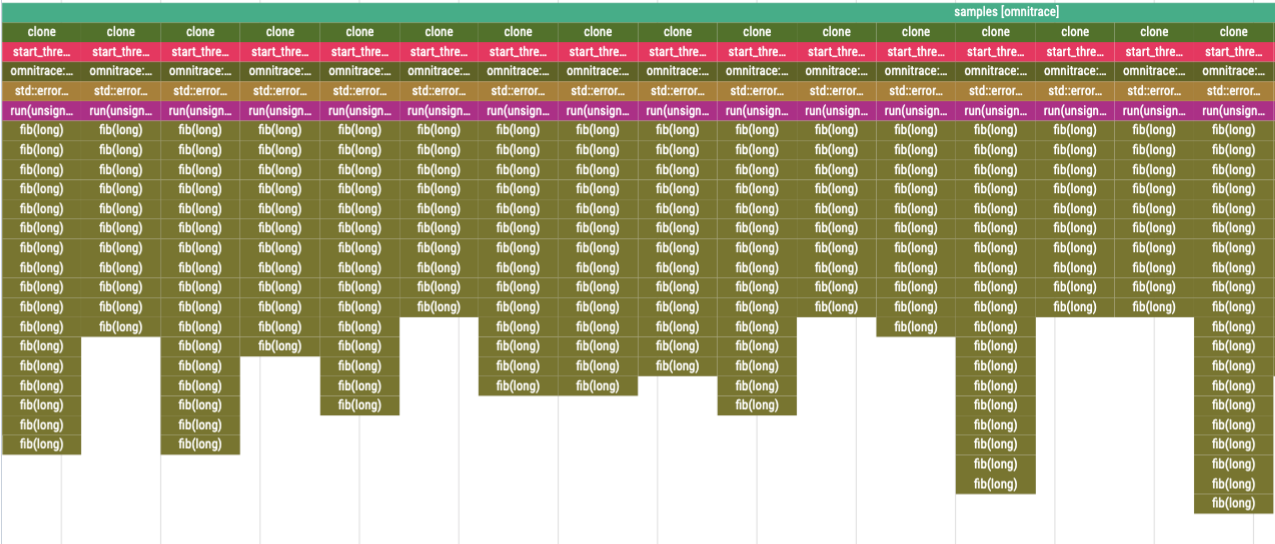
\includegraphics[width=\linewidth]{Appendici/CallStackSampling.png}
        \caption{呼叫堆疊採樣 (call-stack sampling)}
        \label{fig:call-stack-sampling}
    \end{subfigure}

    \begin{subfigure}[b]{\textwidth}
        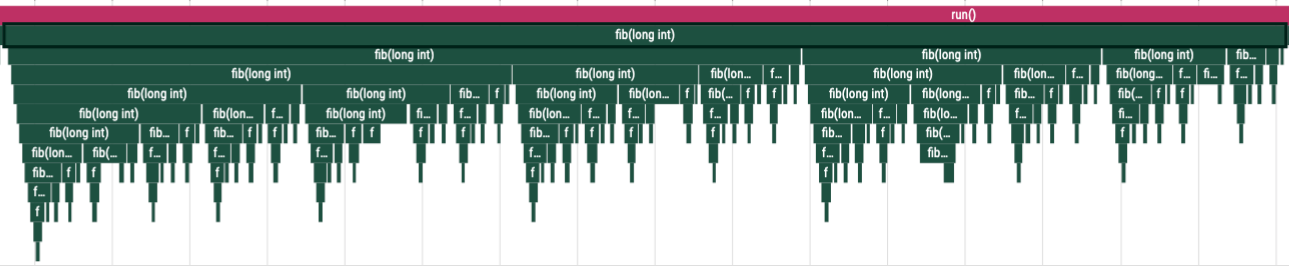
\includegraphics[width=\linewidth]{Appendici/BinaryInstrumentation.png}
        \caption{二進位檔案插樁 (binary instrumentation)}
        \label{fig:binary-instrumentation}
    \end{subfigure}

    \caption{比較使用呼叫堆疊採樣 (call-stack sampling) 和二進位檔案插樁 (binary instrumentation) 在執行遞迴斐波那契數計算程式時所產生的追蹤資料。\\呼叫堆疊採樣方法的解析度有限,無法捕捉精確的函數開始和結束時間。}
    
\end{figure}


無論選擇哪種方法,建議使用者在編譯執行檔時啟用優化 (\lstinline|-O2| 或更高)、禁用 assertion (\lstinline|-DNDEBUG|),並包含除錯資訊(指定 \lstinline|-g1| 或更高的級別)。

\paragraph{呼叫堆疊採樣 (call-stack sampling)}
呼叫堆疊採樣可以透過執行 \lstinline|omnitrace-sample| 執行檔來啟動。例如,如果要執行的 GPU 程式叫做 \lstinline|foo|,以下指令會使用呼叫堆疊採樣來執行 foo:

\lstinline|omnitrace-sample -- foo|

\lstinline|omnitrace-sample| 執行檔使用一般的 LLM 風格命令列參數語法。所有雙連字號 \lstinline|--| 前的參數是給 Omnitrace 的,而 \lstinline|--| 後面的參數則是給程式的。

\paragraph{二進位檔案插樁 (binary instrumentation)}
二進位檔案插樁可以透過執行 \lstinline|omnitrace-instrument| 執行檔來完成,該工具會修改主程式,插入收集追蹤的程式碼。預設情況下,\lstinline|omnitrace-instrument| 會同時插樁並執行程式。其語法與 \lstinline|omnitrace-sample| 類似,\lstinline|omnitrace-instrument| 的參數和程式的參數由雙連字號 \lstinline|--| 分開。

另外,\lstinline|omnitrace-instrument| 也可以連接到正在運行的程序,或者生成已插樁的二進位檔案以供稍後執行。若要連接到正在運行的程序,請使用 \lstinline|-p| 參數,後面跟著程序 ID(PID),如以下指令所示:

\lstinline|omnitrace-instrument <omnitrace-options> -p <PID> -- <exe-name>|

若要創建已插樁的二進位檔案,請使用 \lstinline|-o| 參數來指定輸出的檔案名稱,如以下指令所示:

\lstinline|omnitrace-instrument <omnitrace-options> -o <name-of-new-exe-or-library> -- <exe-or-library>|

如同讀者可能已經注意到,我們並未指定要為哪些函數來收集追蹤資料。這是因為 Omnitrace 有一個預設規則來選擇要插樁的函數。預設情況下,所有函數都會被插樁追蹤,除非函數符合以下條件:1) 動態呼叫位址(例如函數指標),或 2) 少於 1024 個指令。\footnote{有更多規則會防止函數被插樁。請參閱 Omnitrace 文件以獲得更多資訊。}

\lstinline|omnitrace-instrument| 工具提供了三組參數來自訂要插樁的模組(函式庫)與函數。\lstinline|--module-include| 和 \lstinline|--function-include| 參數分別允許使用者加入預設插樁規則以外的模組和函數。這些參數可以使用正規表達式來匹配模組和函數名稱。相對地,\lstinline|--module-restrict| 和 \lstinline|--function-restrict| 參數則會覆寫預設的選擇,只包含與提供的正規表達式匹配的模組和函數。最後,\lstinline|--module-exclude| 和 \lstinline|--function-exclude| 參數讓使用者能夠調整選擇,將一些預設的模組和函數排除。

\subsection{輸出與視覺化}
Omnitrace 的輸出會儲存於以下路徑:

\lstinline|<OUTPUT_PATH>[/<TIMESTAMP>]/[<PREFIX>]<DATA_NAME>[<OUTPUT_SUFFIX>].<EXT>|

透過設定一些環境變數,我們可以指定資料追蹤的輸出位置與檔案名稱。例如,\lstinline|OMNITRACE_OUTPUT_PATH| 環境變數可以用來指定儲存輸出檔案目錄的路徑。在路徑中,使用者可以插入特殊的佔位符號來描述追蹤資料的內容。這些佔位符號包括 \lstinline|%argt%|、\lstinline|%ppid%|、\lstinline|%pid%| 和 \lstinline|%rank%|,分別代表執行檔的 basename、父程序 ID、程序 ID 和 MPI rank。若要查看完整的選項列表,包含其描述,使用者可以執行指令 \lstinline|omnitrace-avail –list-keys –expand-keys|

每次執行 Omnitrace 時,會生成一個 \lstinline|perfetto-trace.proto| 的檔案。該檔案可以透過 Perfetto 視覺化工具來開啟,該工具可於以下網址取得:\url{ui.perfetto.dev}(參見圖 \ref{fig:omnitrace-visualization} 查看範例)

\begin{figure}
    \centering
    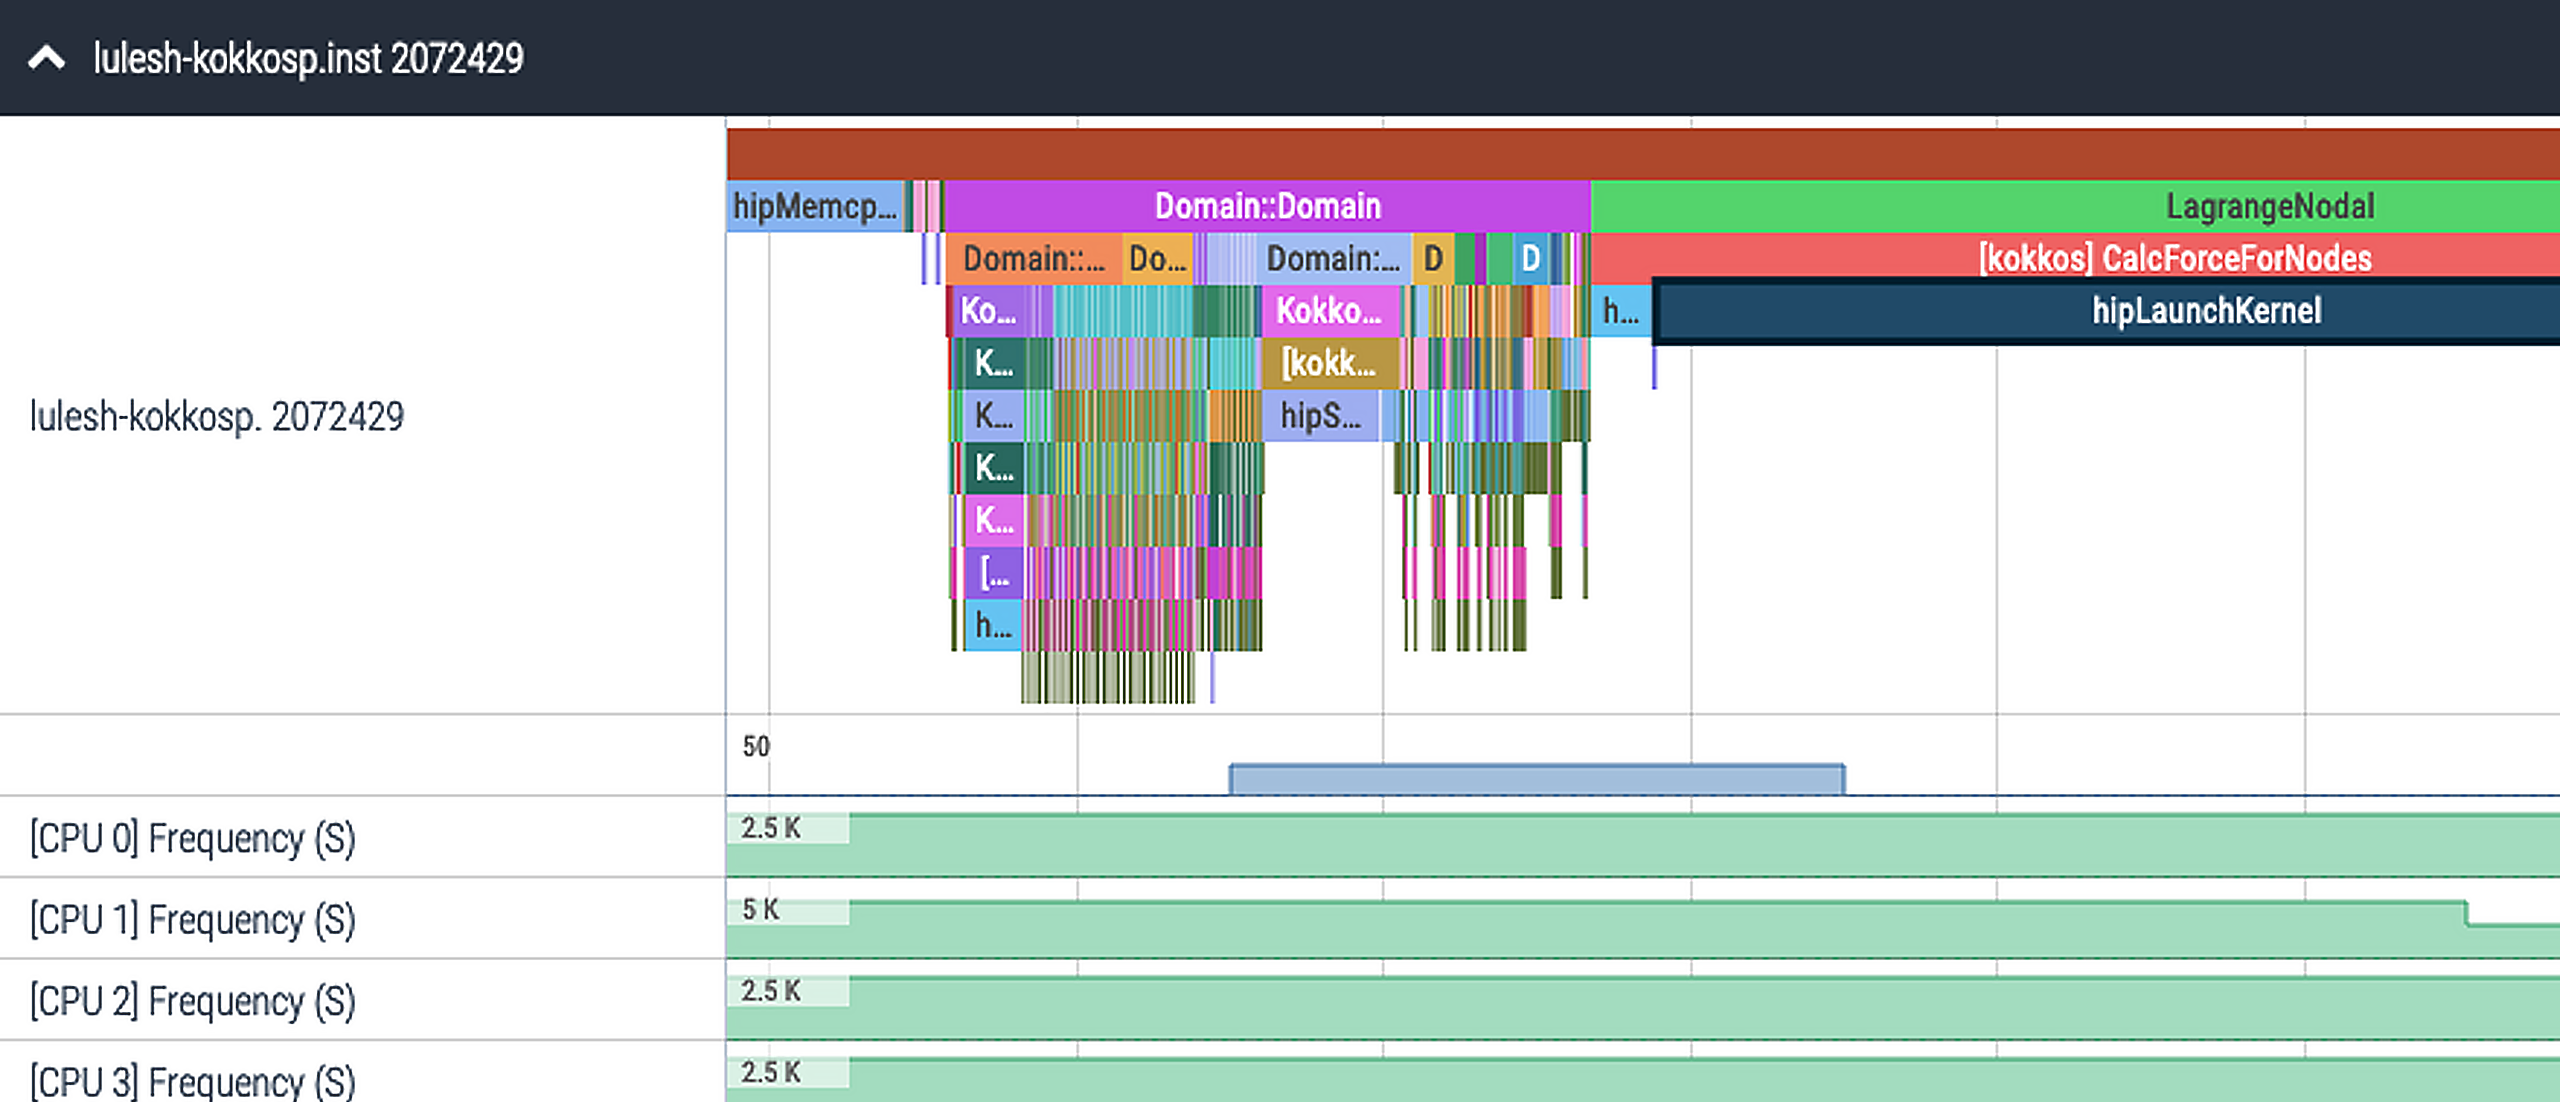
\includegraphics[width=1\linewidth]{Appendici/OmnitraceVisualization.png}
    \caption{使用 Omnitrace 生成的追蹤資料視覺化的範例}
    \label{fig:omnitrace-visualization}
\end{figure}


\section{Omniperf}

相對於專注於主機端函數呼叫剖析的 Omnitrace,Omniperf 提供了 kernel 層級的剖析功能。Omniperf 基於 rocProf 開發,能夠對在 AMD Instinct MI GPU(例如 MI100、MI200 和 MI300 系列 GPU)上運行的機器學習(ML)和高效能運算(HPC)的工作進行剖析。

Omniperf 擁有全面的功能,提供各種面板來做深入的分析,包括 System Speed-of-Ligh 與  Memory Chart Analysis。該工具同時支援命令列和圖形使用者介面(GUI)分析,以滿足不同使用者的需求,並增強對效能資料的整體取得能力。


\subsection{使用 Omniperf 剖析程式}
Omniperf 的核心是一個可以以剖析模式啟動程式的命令列工具。假設我們的 GPU 程式名為 \lstinline|vcopy|,以下指令可以收集程式中所有 kernel 的所有可用計數器:

\lstinline|omniperf profile -n vcopy_data -- ./vcopy -n 1048576 -b 256|

與 Omnitrace 類似,雙連字號 \lstinline|--|用來分隔 Omniperf 的參數和我們想要剖析的程式名稱。Omniperf 的 \lstinline|-n| 參數定義了輸出的目錄名稱。在這個例子中,輸出將會儲存在目錄 \lstinline|./workloads/vcopy_data/MI200| 中。值得注意的是,除非使用 \lstinline|-p|/\lstinline|--path| 參數來覆寫輸出路徑,Omniperf 會將加速器的名稱附加為目錄的最後一層。

收集所有 kernel 的追蹤資料是非常耗時的。由於硬體效能計數器的數量有限,通常需要多次重新執行 kernel 才能收集所有的指標。為了減少收集特定指標的執行時間,Omniperf 提供了幾個參數,包括:

\begin{itemize}
\item \lstinline|-k|/\lstinline|--kernel| 可以根據 kernel 的名稱過濾 kernel。
\item \lstinline|-d|/\lstinline|--dispatch| 可以根據 dispatch ID(即第 n 個派遣的 kernel)過濾 kernel。
\item \lstinline|-b|/\lstinline|--block| 可以根據硬體元件區塊 (hardware component blocks) 過濾指標。
\end{itemize}

除了除錯典型的效能瓶頸外,Omniperf 還可以用來生成用來做 roofline 分析的指標 \cite{williams2009roofline}。如果不需要收集 roofline 分析的指標,可以透過指定 \lstinline|--no-roof| 來讓 Omniperf 執行而不收集相關的剖析資料。或者,我們也可以選擇加入 \lstinline|--roof-only| 參數來只剖析 roofline 分析的指標。

使用 empirical roofline model, 使用者可以視覺化比較應用程式的實際效能與機器的最大可達效能。Omniperf 的 roofline 分析功能會直接生成 roofline 視覺化圖表,並以 PDF 格式輸出(請參見圖 \ref{fig:roofline1} 和圖 \ref{fig:roofline2})。

\begin{figure}
    \centering
    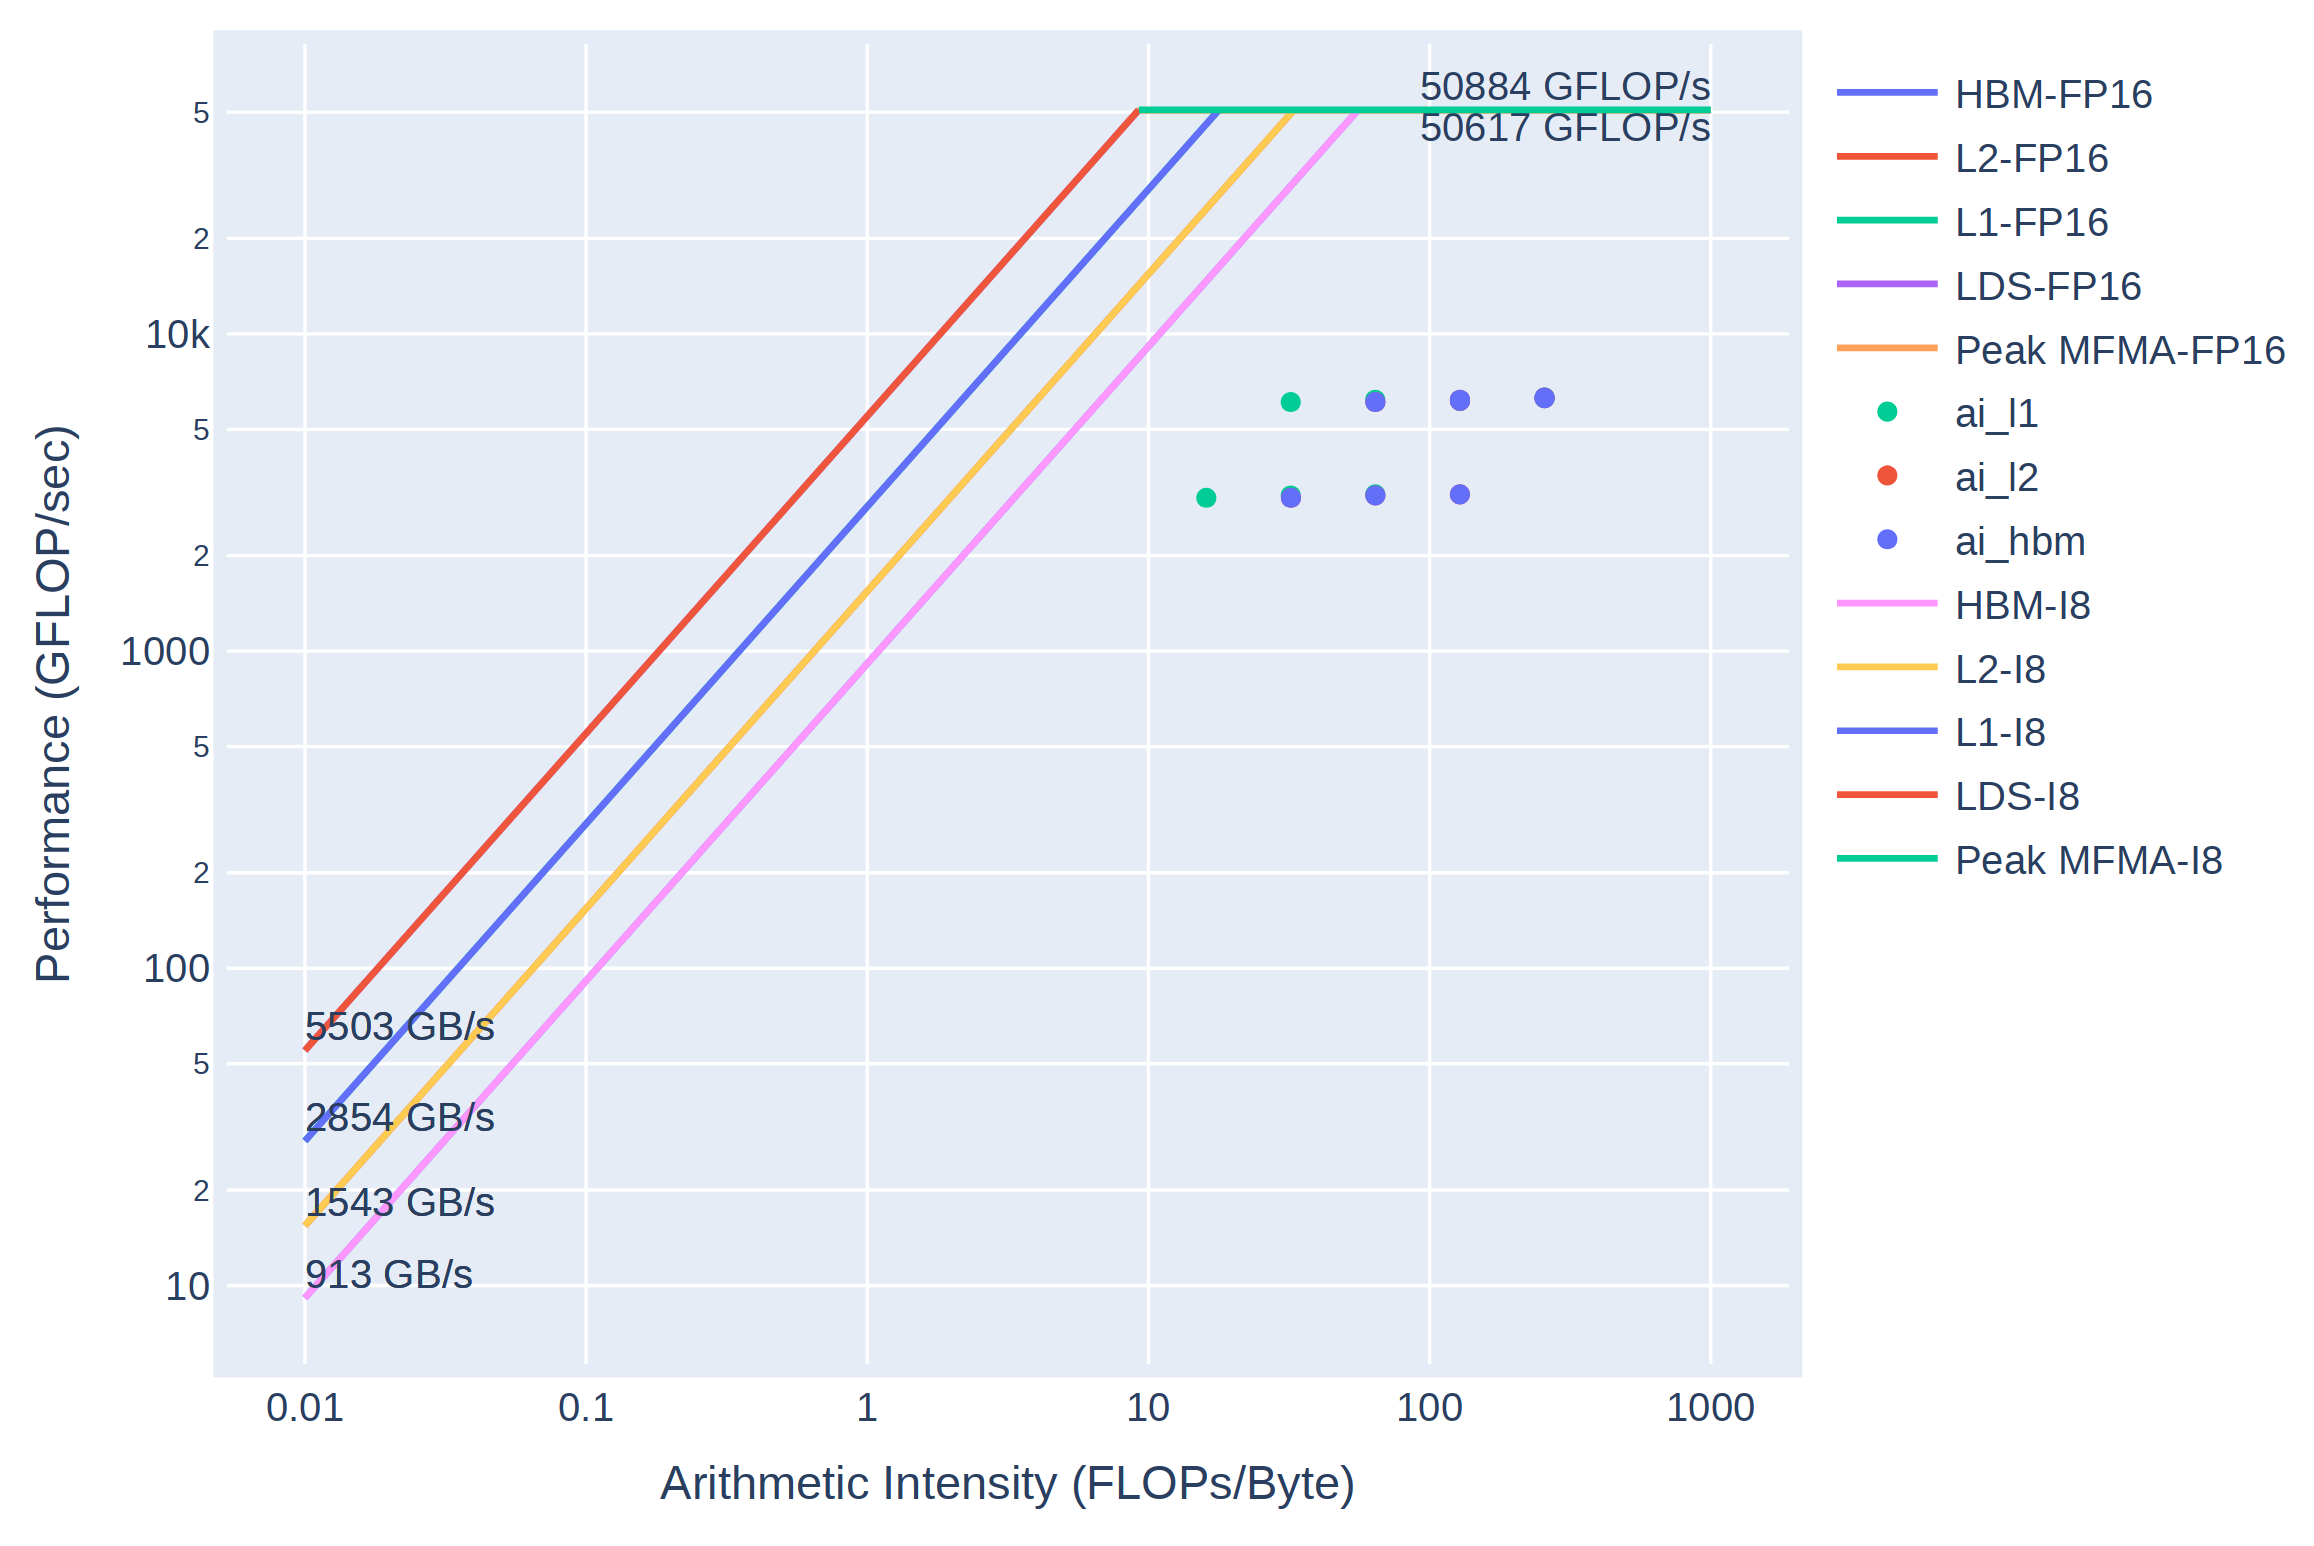
\includegraphics[width=1\linewidth]{Appendici/Roofline1.png}
    \caption{8 位元整數與 16 位元浮點運算的 roofline 分析圖表}
    \label{fig:roofline1}
\end{figure}

\begin{figure}
    \centering
    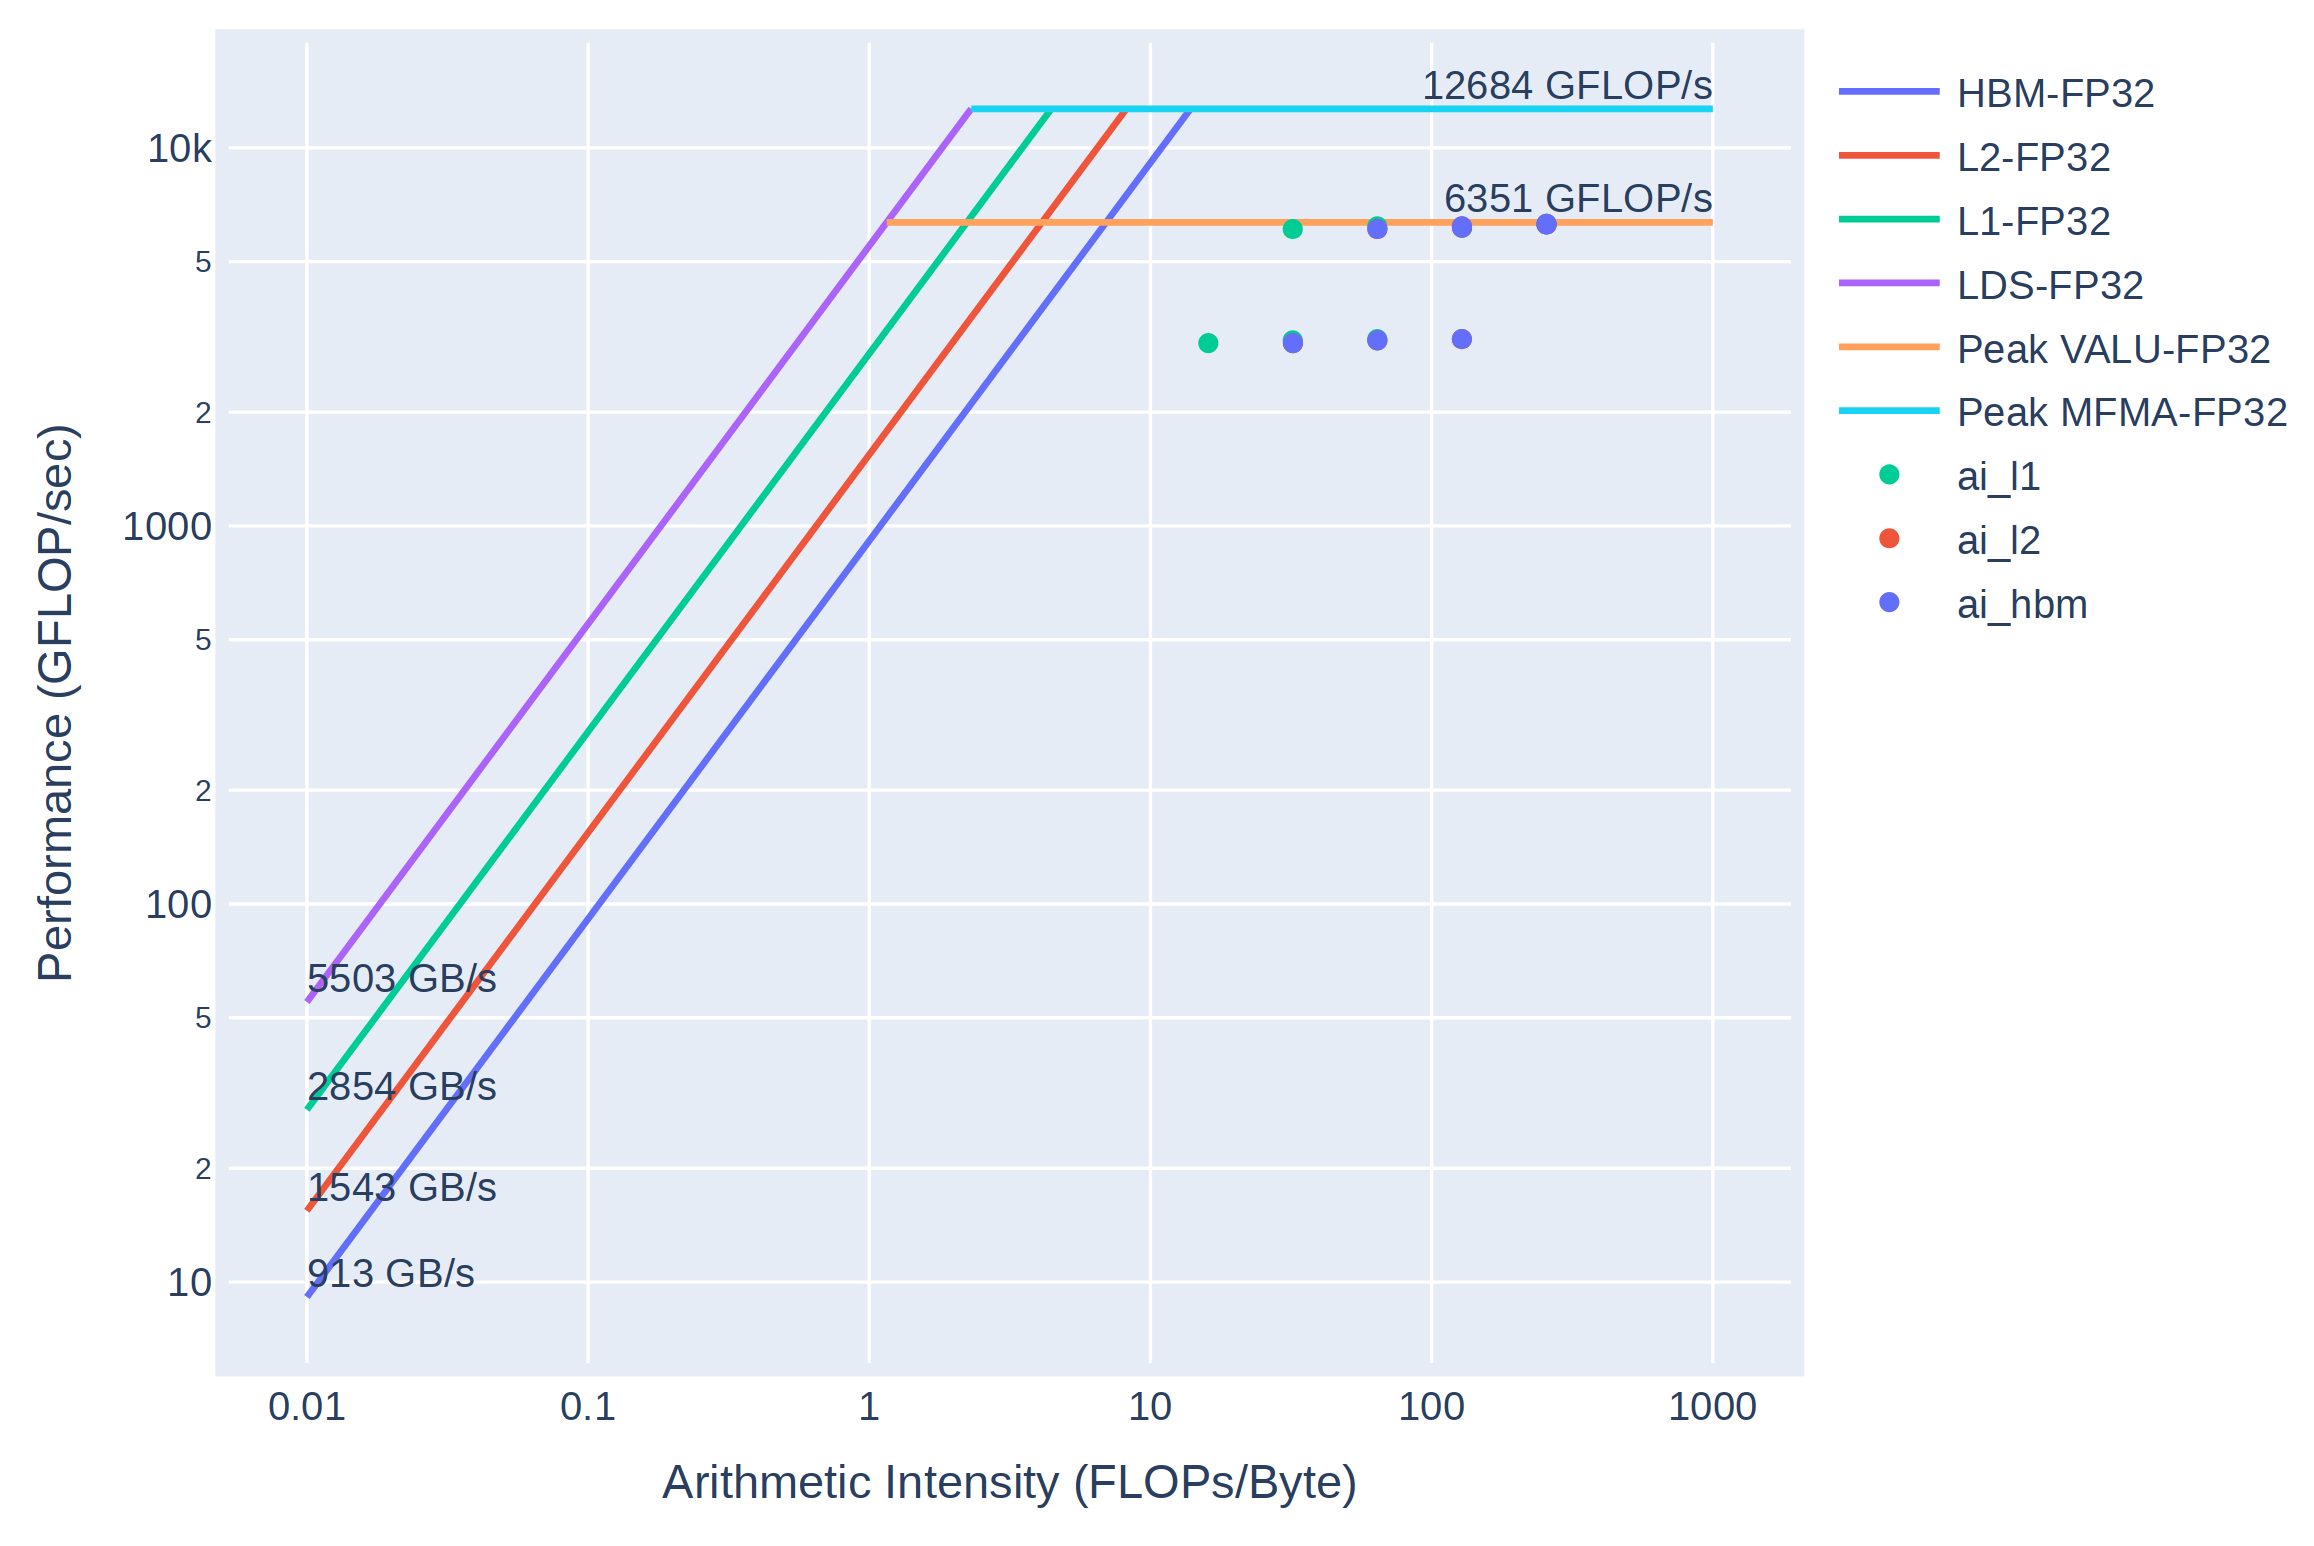
\includegraphics[width=1\linewidth]{Appendici/Roofline2.png}
    \caption{32 位元整數與 64 位元浮點運算的 roofline 分析圖表}
    \label{fig:roofline2}
\end{figure}

\subsection{使用命令列介面進行分析}
收集的原始剖析資料對大多數使用者來說不容易解讀。為了解決這個問題,Omniperf 提供了一個分析工具,該工具會處理資料來簡化詮釋的過程。這個分析工具也內建於 \lstinline|omniperf| 命令列工具中。我們可以使用以下指令來啟動此工具:

\lstinline|omniperf analyze -p workloads/vcopy/MI200/|

在這裡,參數 \lstinline|-p| 需要提供在剖析階段時收集的原始指標的路徑。

分析工具會將處理後的資料以表格形式顯示在命令列介面中(參見圖 \ref{fig:omniperf-cli})。輸出通常包含三個部分,包含高層次的狀態資訊(kernel 與其執行時間)、系統資訊以及系統的 Speed-of-
Light 分析(即衍生的效能指標)。衍生的效能指標通常是能夠自我解釋的,但使用者仍然可以參考 Omniperf 文件來獲得更詳細的解釋。\footnote{\url{https://rocm.github.io/omniperf/performance_model.html}}

此外,Omniperf 的命令列介面分析工具也支援比較兩次不同的執行結果。假設原始剖析輸出儲存在 \lstinline|workload1/path| 和 \lstinline|workload2/path|,我們可以使用以下指令來比較它們:

\lstinline|omniperf analyze -p workload1/path -p workload2/path|

Omniperf 的分析工具可以並排顯示衍生的效能指標,以方便比較(參見圖 \ref{fig:omniperf-compare})。

\begin{figure}
    \centering
    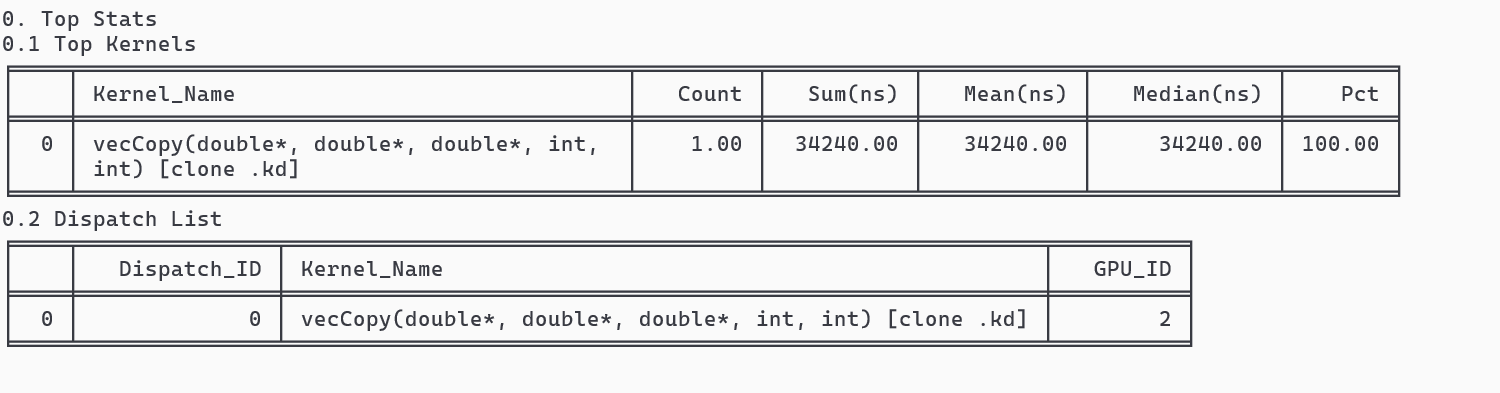
\includegraphics[width=1\linewidth]{Appendici/OmniperfCLI.png}
    \caption{命令列介面分析工具輸出的開始部分}
    \label{fig:omniperf-cli}
\end{figure}

\begin{figure}
    \centering
    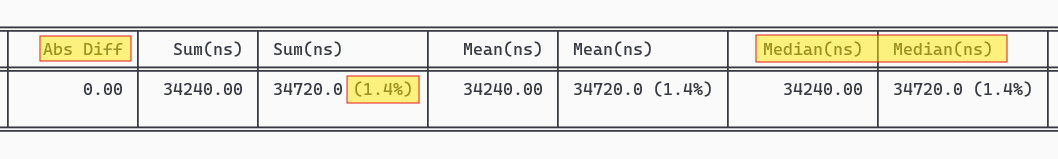
\includegraphics[width=1\linewidth]{Appendici/OmniperfCompare.png}
    \caption{Omniperf 分析工具在比較兩次執行時的輸出。Count、Sum、Mean 和 Median 等欄位會顯示兩次,第二次顯示的是 workload 2 的資料。相對差異也會顯示在 workload 2 的欄位中。}
    \label{fig:omniperf-compare}
\end{figure}


\subsection{使用基於網頁的 GUI 進行分析}
為了提供更使用者友善的效能分析介面,Omniperf 可以啟動一個基於 Flask \cite{grinberg2018flask} 的網頁伺服器。使用者可以透過網頁瀏覽器來檢視結果。只需要在 \lstinline|omniperf analyze| 指令中加入 \lstinline|--gui| 參數,如下指令所示:

\lstinline|omniperf analyze -p workloads/vcopy/MI200 --gui|

開啟網頁介面的 URL 會顯示在終端機中(如 \url{http://127.0.0.1:8050})。預設情況下,Omniperf 使用 8050 連接埠。

網頁介面(參見圖 \ref{fig:omniperf-web-interface})包括一個控制面板(上方)、記憶體分析面板(中間)和 roofline 分析面板(底部)。使用者可以使用下拉選單來過濾分析結果,選擇特定的 kernel 與要關注的 kernel dispatch。

\begin{figure}
    \centering
    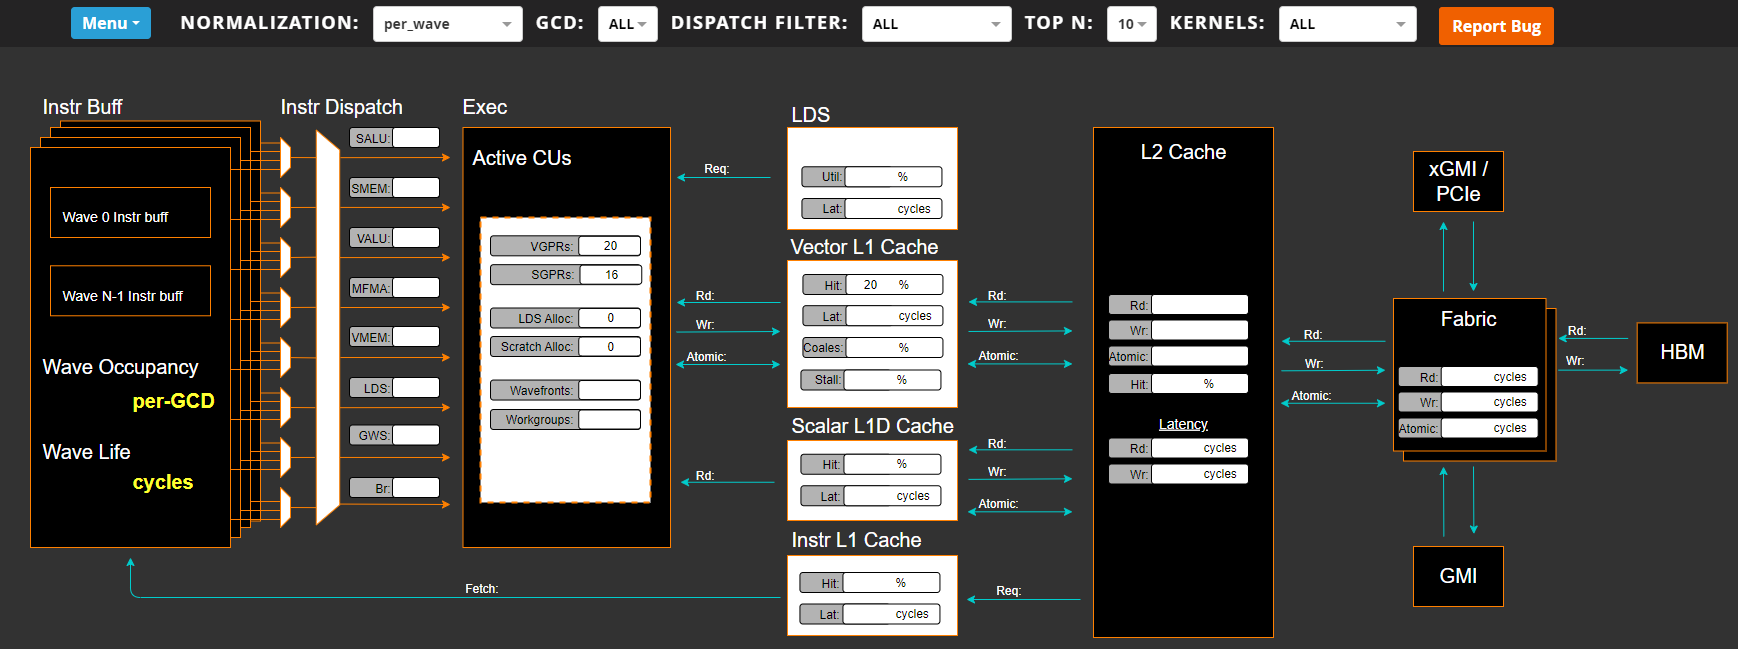
\includegraphics[width=1\linewidth]{Appendici/OmniperfWebInterface}
    \caption{基於網頁的 Omniperf 分析 GUI 介面}
    \label{fig:omniperf-web-interface}
\end{figure}


\subsection{使用 Grafana 進行分析}
儘管簡單的基於網頁的 GUI 提供了更具使用者友善的效能分析介面,但呈現的資料仍然有限。為了進行全面的 GUI 基礎效能分析,Omniperf 使用了 Grafana \cite{chakraborty2021grafana},一個受歡迎的資料視覺化框架。Grafana 需要將資料儲存於 MongoDB 資料庫中。因此,Omniperf 提供了一個工具,可以使用以下命令將原始指標匯入 MongoDB 資料庫:

\lstinline|omniperf database --import -H 127.0.0.1 -u temp -t asw -w workloads/vcopy/mi200|

這邊的參數 \lstinline|-H| 和 \lstinline|-u| 分別接受 MongoDB 實例的主機 IP 位址與使用者名稱。\lstinline|-t|(team)和 \lstinline|-w|(workload)是用來決定資料庫名稱的參數。預設情況下,資料庫名稱為:

\lstinline|omniperf_<team>_<workload>_<soc>|(如 \lstinline|omniperf_asw_vcopy_mi200|)。

基於 Grafana 的分析工具有 18 個面板,每個面板表示不同類型的資料,以滿足使用者的各種需求。在這一節中,我們展示兩種不同的視圖:1) 指令混合面板(Instruction Mix Panel)與 2) L1 快取面板(L1 Cache Panel)
指令混合面板(參見圖 \ref{fig:instruction-mix-panel})顯示每個 wavefront 的平均指令數量,而 L1 快取面板(參見圖 \ref{fig:l1-cache-panel})顯示 L1 快取命中率和頻寬使用率。欲了解更詳細的資訊和設定說明,讀者可以參考 Omniperf 的 Grafana 設定指南\footnote{\url{https://rocm.github.io/omniperf/installation.html#setup-grafana-instance}}。

\begin{figure}
    \centering
    \begin{subfigure}[b]{\textwidth}
        \centering
        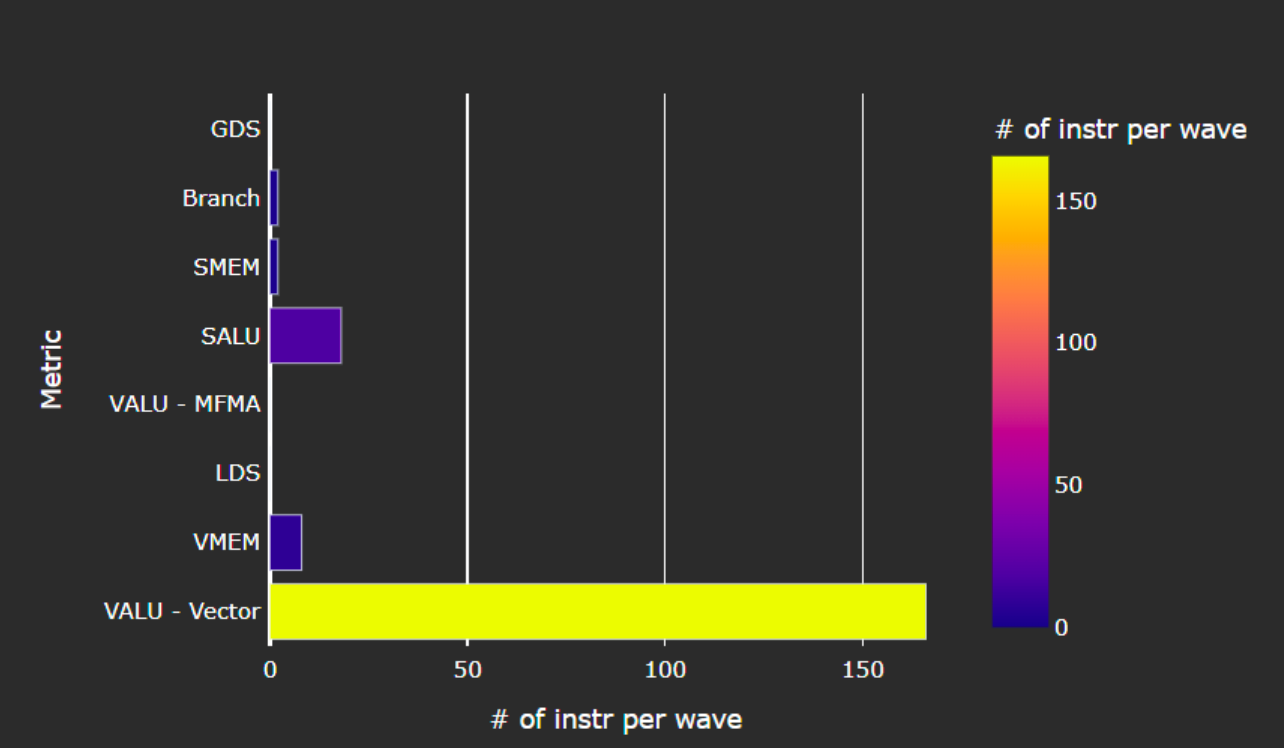
\includegraphics[width=0.5\linewidth]{Appendici/InstructionMixPanel.png}
        \caption{指令混合面板 (Instruction Mix Panel) 顯示每個 wavefront 中每種指令類型的平均數量}
        \label{fig:instruction-mix-panel}
    \end{subfigure}

    \begin{subfigure}[b]{\textwidth}
        \centering
        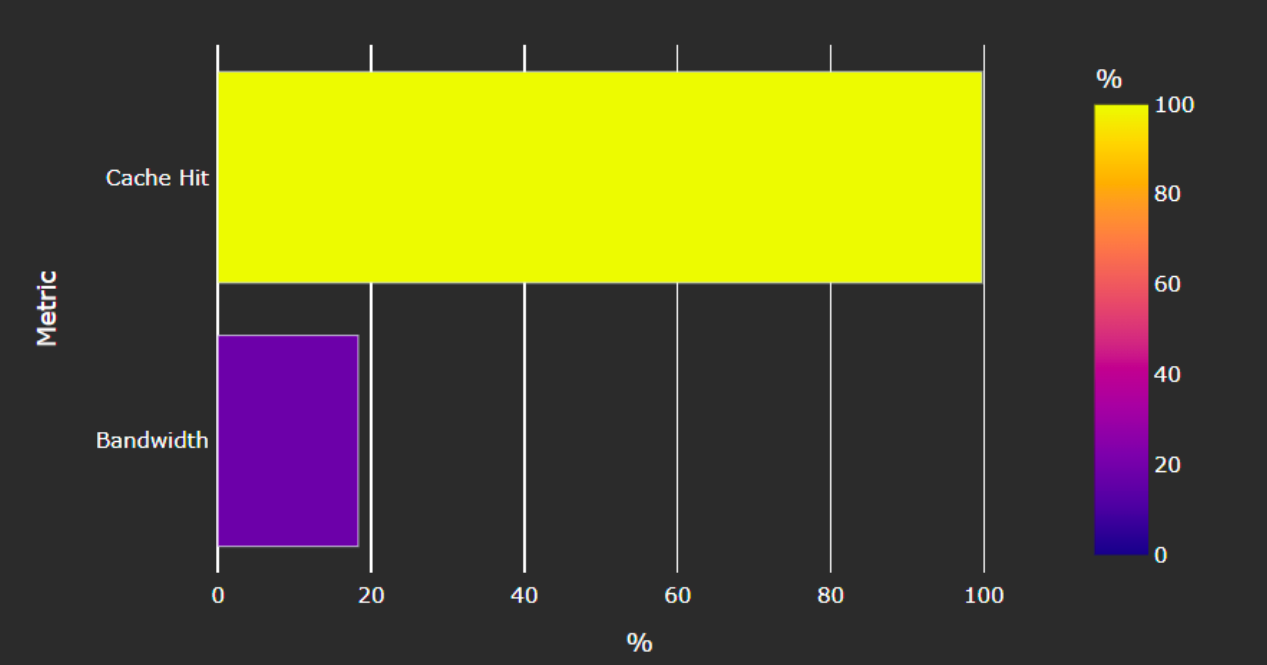
\includegraphics[width=0.5\linewidth]{Appendici/L1CachePanel.png}
        \caption{L1 快取面板 (L1 Cache panel) 顯示快取命中率和頻寬使用率。}
        \label{fig:l1-cache-panel}
    \end{subfigure}

    \caption{Omniperf 中基於 Grafana 的分析工具所提供的範例視圖}
    
\end{figure}

\section{總結}
在本附錄章節中,我們介紹了兩個進階的效能分析工具:1) Omnitrace 與 2) Omniperf。這些工具擴展了內建 ROCm 工具(rocTracer 和 rocProfiler)的功能,提供了捕捉程式執行追蹤和效能指標的能力。Omnitrace 和 Omniperf 提供了額外的分析和視覺化選擇,簡化了優化程式效能的過程。


%%%%%%%%%%%%%%%%%%%%%%%%%%%%									BACKMATTER
%%%%%%%%%%%%%%%%%%%%%%%%%%%%
\backmatter

%%%%% 							BIBLIOGRAFIA
\pagestyle{fancyBibliografia}
\titleformat{\chapter}
	[hang]
	{\vspace{-2cm}\Huge}
	{}
	{0em}
	{}
	[\Large {\begin{tikzpicture} [remember picture, overlay]
	\pgftext[right,x=14.75cm,y=0.2cm]{\HUGE\bfseries 
	Bibliography}
	\end{tikzpicture}}]
	
	\nocite{*}
	\bibliographystyle{amsalpha}
	\bibliography{FileAusiliari/Bibliografia}
	\addcontentsline{toc}{part}{Bibliography}
\cleardoublepage
%INDICE ANALITICO
\begin{comment}
 \pagestyle{fancyIndiceAnalitico}
 	\renewcommand{\indexname}{}
	% SISTEMA IL PROBLEMA DEL LINK ALL'INDICE ANALITICO
	\let\cleardoublepage\relax
	\titleformat{\chapter}[hang]{}{}{0em}{}[]
 	\chapter*{}
	\titleformat{\chapter}
		[hang]
		{\Huge}
		{}
		{0em}
		{}
		[\Large {\begin{tikzpicture} [remember picture, overlay]
		\pgftext[right,x=14.75cm,y=0.2cm]{\HUGE\bfseries 
			Indice analitico}
		\end{tikzpicture}}]
	\titlespacing*{\chapter}{0pt}{0\baselineskip}{5\baselineskip}
	\addcontentsline{toc}{part}{Indice analitico}	
	\vspace{-2cm}
	\printindex
    \end{comment}
%%%%%%%%%%%%%%%%%%%%%%%%%%%%%%%%%%%%%%%%%%%%%%%%%%%%%%%%%%%%%%%%%%%%%%%%%%%%%%%%%%%%%%%%%%%%%%%%%%%%%%%%%%%%%%%%%
\end{appendices}
\end{document}